\section{Practice}
\label{sec:experiments}

This section will provide the implementation details of the theory part (Section \ref{sec:theory}). The algorithm is implemented in C ++ and makes use of the CGAL library (\url{https://www.cgal.org}). 
Then, given the implementation, experimental setups will be introduced. The experimental setup will include some basic test polygons to check the correct execution of the algorithm. We will also observe the behaviour of the algorithm and emphasise the importance of each of the heuristics used. Lastly, we will showcase the fragility and importance of hyperparameters.

Polygons used:
- 2 guards
- random
- love
- comb
- corridor

For every heuristic:
- show how each polygon behaves when turning it off

Try to see if the comb polygon scales

\subsection{Heuristics}
In this subsection we will observe the role played by each of the heuristics used. We will additionally notice how different heuristics are more relevant for different types of polygons. In order to do so, we will run the program with all of the heuristics but one, for each of the heuristics. By analysing the difference in movement for each of the guards', we will be able to assess the influence every heuristic has on each type of polygon.

We will use fixed hyperparameters for all the runs. This will allow us to focus on the differences between the heuristics. Later in this section we will also discuss the actual hyperparameter choice. As such, we will use a momentum past weight $\gamma = 0.8$ and pull attraction $\beta = 1$. The learning rate will be varied per polygon and type of experiment. This choice is due to the fragility of the algorithm implementation and will be explained later in this section.

\subsubsection{Without Momentum}
In this section we will discuss the impact momentum has on the overall behaviour of the algorithm. As introduced in Section \ref{sec:momentum}, momentum takes into account the position history of the guards. In this way, the overall trajectory of a guard is smoothened out.

A suggestive way to observe this is with the arbitrary polygon from Figure \ref{fig:random}. The polygon requires a minimum of 3 guards to be fully seen. For this reason, we will run the algorithm with only 3 guards.

\begin{figure}[h!]
    \centering
    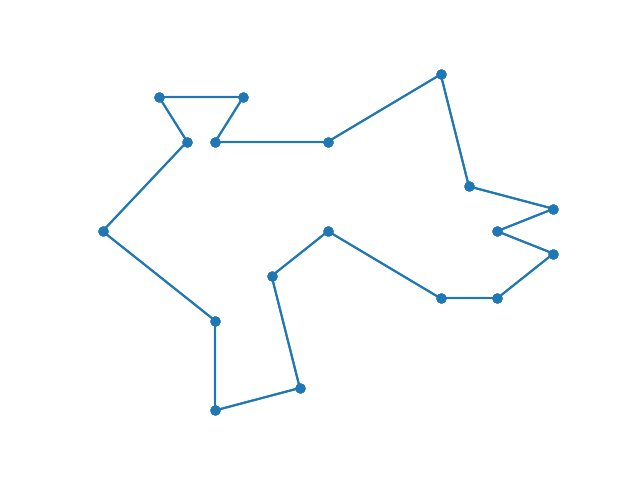
\includegraphics[width = 0.5\textwidth]{experiments/random.png}
    \caption{Arbitrarily shaped polygon.}
    \label{fig:random}
\end{figure}

We will compare how the guards move when we are using all the heuristics to when we are not using momentum. The guards will have a learning rate $\alpha = 0.2$. They will start at the same fixed position in both cases.

Figure \ref{fig:no_momentum} displays the area seen per iteration for the arbitrary polygon Both the total area seen and the individual area seen by each are shown. Starting with almost the whole area seen, the guards are eventually optimally placed in a position from which the whole polygon is seen. Nonetheless, using momentum clearly makes a difference in Subfigure \ref{fig:no_momentum1}, than when not using it in Subfigure \ref{fig:no_momentum2}. Using momentum allows the overall seen area to keep a steady trajectory towards its maximum. Additionally, guards quickly find their optimum in only 4 iterations, without many oscillations. In Subfigure \ref{fig:no_momentum2} however we can observe how the total area fluctuates. The guards also display large jumps close to iterations 5 and 20. These jumps cause the overall progress towards the optimum to be less stable. For example, when guard 2 has a sudden drop in the area it sees around iteration 5, the total area seen naturally drops as well, and only recovers after iteration 20, when guard 0 makes another large jump. This behaviour also suggests that the movement of one guard can heavily influence others, resulting in a noisy behaviour and in a higher number of iterations.
% Subfigure \ref{fig:no_momentum1} displays a more smoothened out trajectory for each guard. 
Therefore, it becomes clearer how momentum allows the smoothening of noisy guard movements. Additionally, we reckon that because guards are holding a steadier trajectory, they are more likely to achieve the optimum in less iterations (in this example, 3). When not using momentum, the number of iterations increases substantially to 24. Momentum thus is a crucial improving heuristic to our whole algorithm, both in speedup as well as in the smootheness of the process.

\begin{figure}[h!]
    \centering
    \begin{subfigure}{0.45\textwidth}
        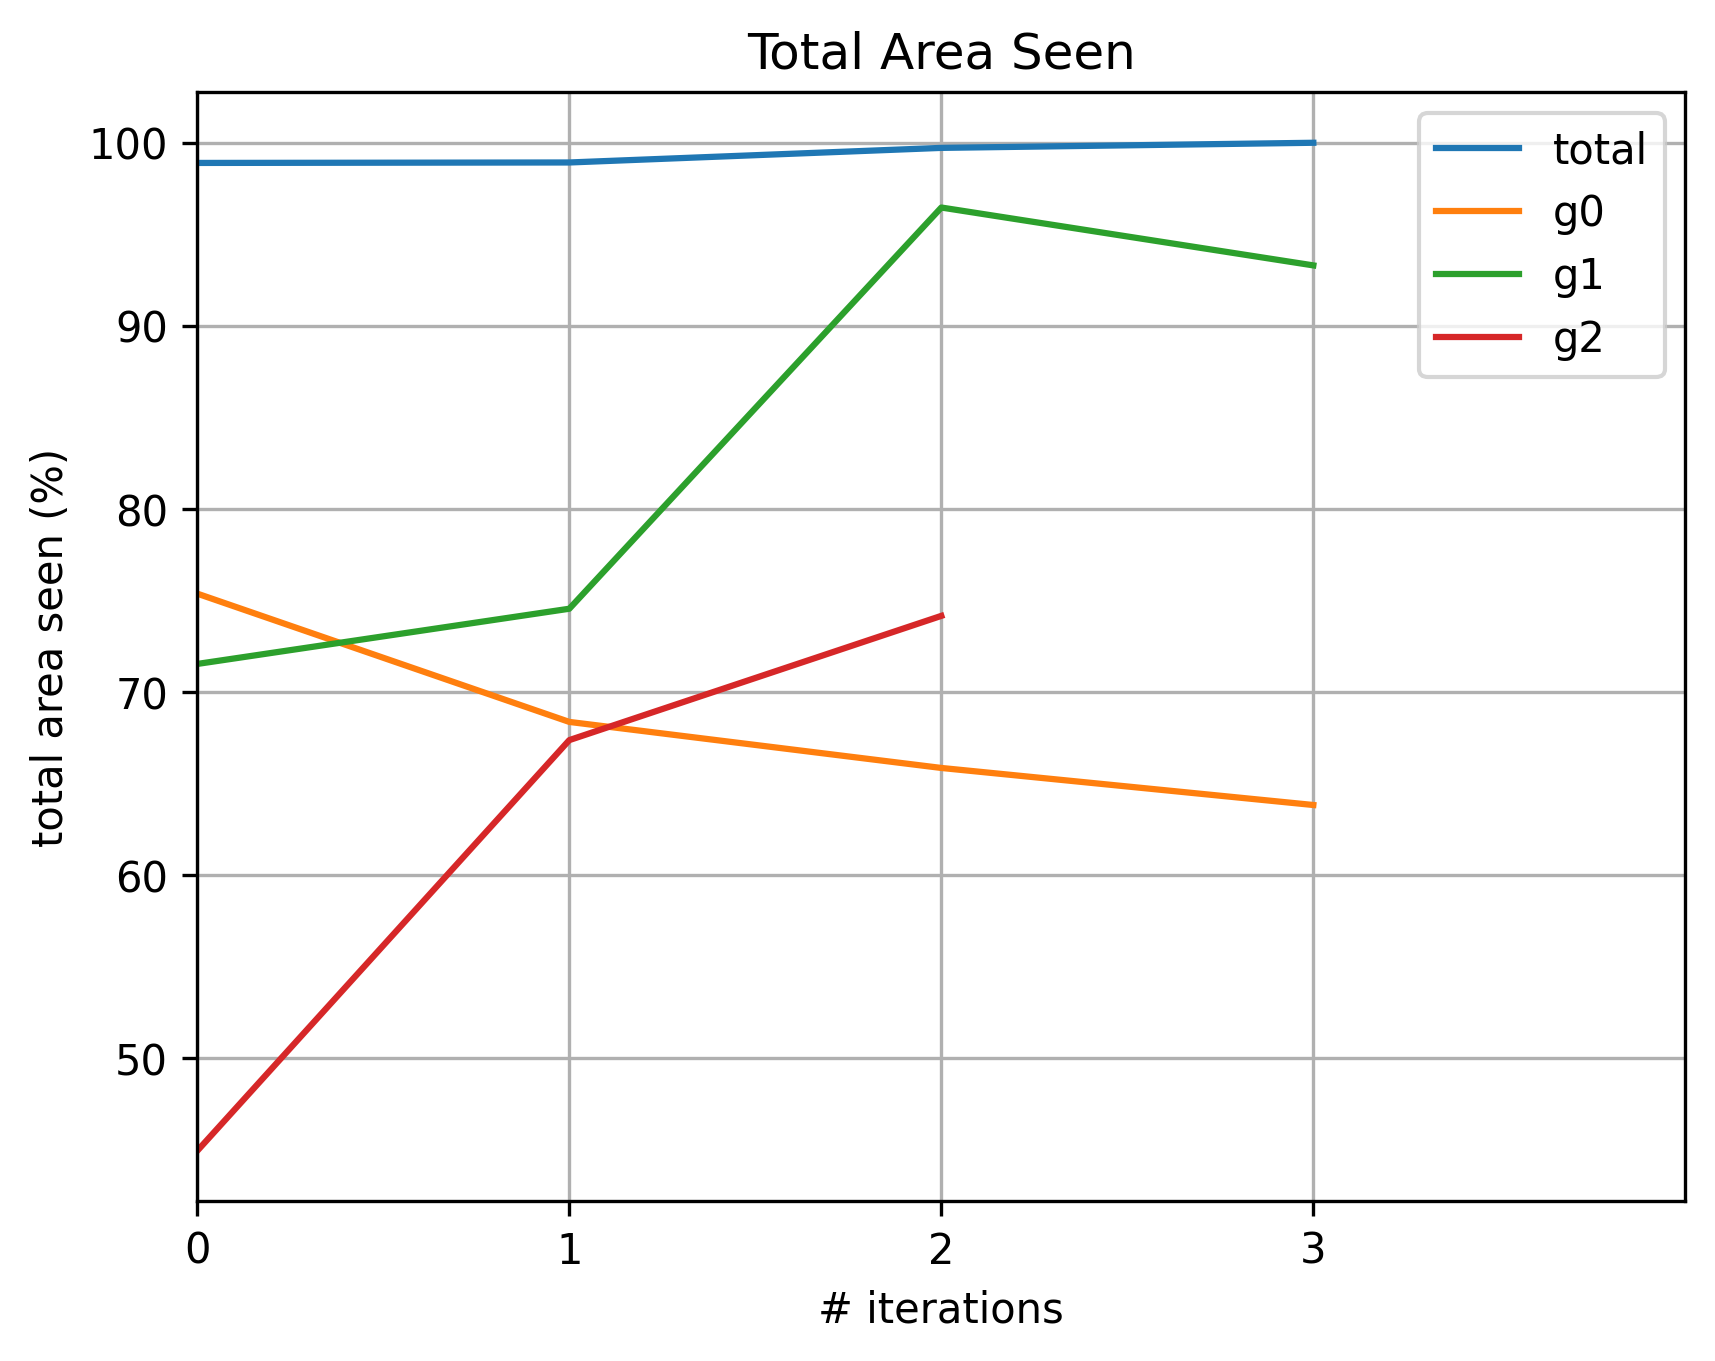
\includegraphics[width = \textwidth]{experiments/area_random_all.png}
        \caption{All heuristics.}
        \label{fig:no_momentum1}
    \end{subfigure}
    \begin{subfigure}{0.45\textwidth}
        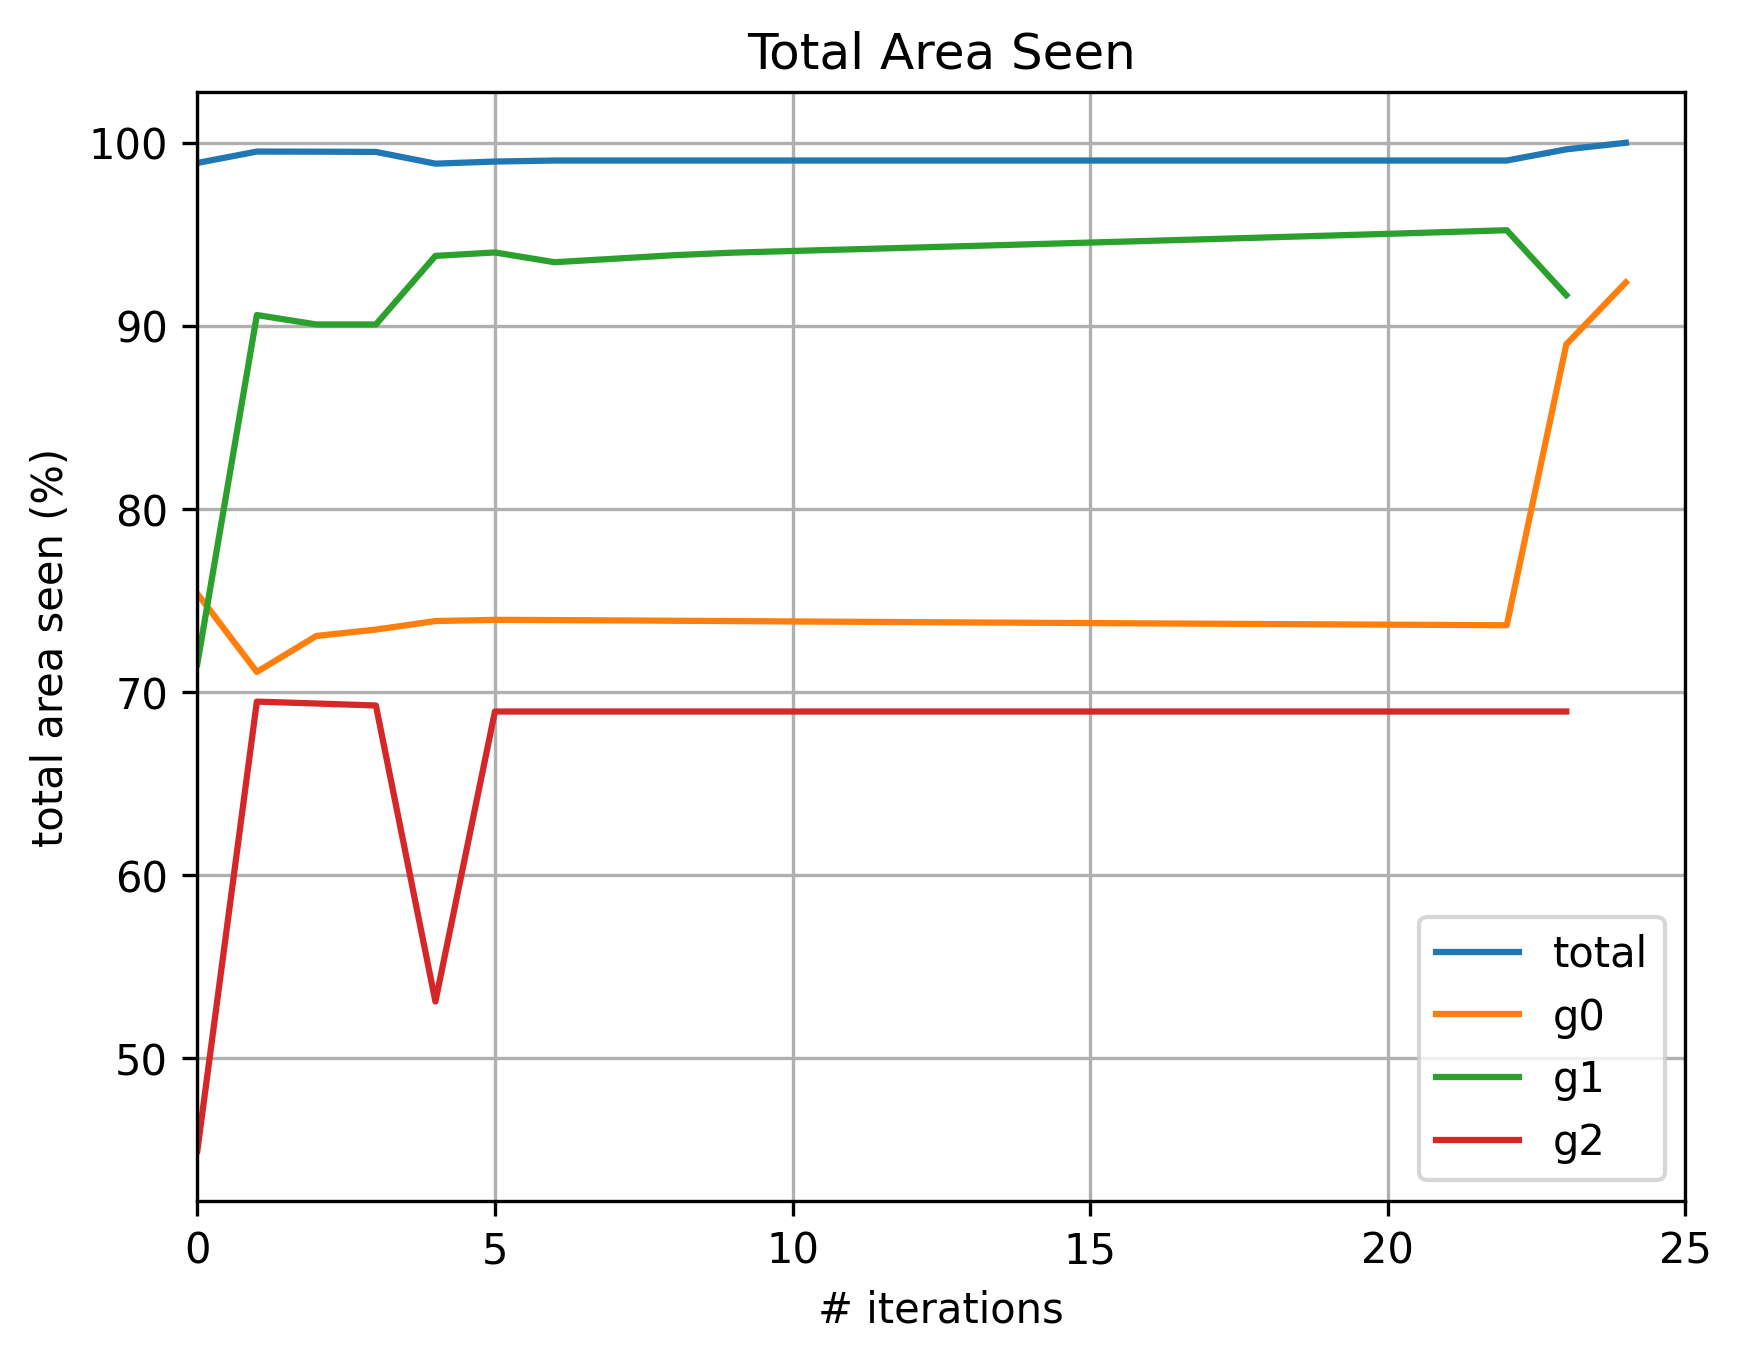
\includegraphics[width = \textwidth]{experiments/area_random_no_momentum.png}
        \caption{No momentum.}
        \label{fig:no_momentum2}
    \end{subfigure}
    \caption{Total area seen per iteration for an arbitrary polygon guarded by 3 guards.}
    \label{fig:no_momentum}
\end{figure}

\subsubsection{Without Line Search}
In this section we will discuss the impact line search has on the overall behaviour of the algorithm. As introduced in Section \ref{sec:line_search}, line search determines how far a guard should move into the optimal direction. In this way, it computes the optimal position of a guard on the direction line given a step size.
In our experiments, the search will compute the best guard placement between multiple positions computed from movement factor $\frac 1 32$ to 32 with a step size $s = 2$.

A suggestive way to observe how well Line Search works is with the comb polygon with four teeth from Figure \ref{fig:comb}.

\begin{figure}[h!]
    \centering
    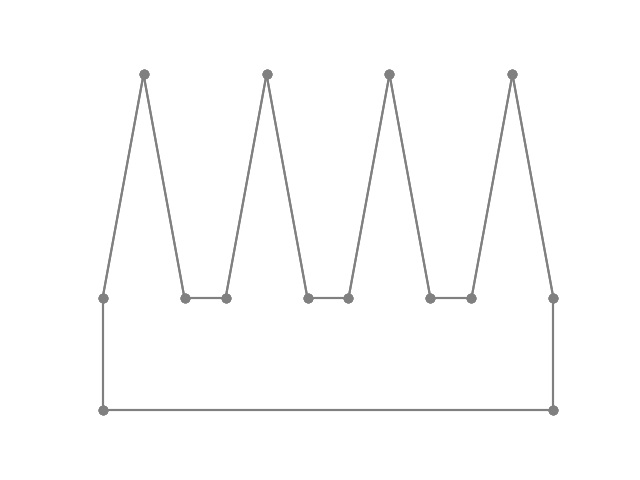
\includegraphics[width = 0.5\textwidth]{experiments/comb.png}
    \caption{Polygon in the shape of a comb with four teeth.}
    \label{fig:comb}
\end{figure}

We will compare how the guards move when we are using all the heuristics to when we are not using line search. The guards have a learning rate $\alpha = 0.4$. They will start at the same fixed position in both cases.

Figure \ref{fig:no_line_search} displays the area seen per iteration for the comb polygon with four teeth. Both the total area seen and the individual area seen by each guard are shown. Starting with around 82.5\% total area seen, the guards are eventually optimally placed in a position from which the whole polygon is seen. Nonetheless, using line search clearly makes a difference between Subfigures \ref{fig:no_line_search1} and \ref{fig:no_line_search2}. The first noticeable difference is the number of iterations. Using line search allows the guards to find their optimal positions in 3 iterations, with a steady increase in the total area seen. On the other hand, not using line search results in the optimal position to be found in more than 80 iterations. What is more, 3 of the guards seem to have found their optimal position after the $30^{\text{th}}$ iteration, whereas the last 50 iterations are spent on only one guard finding its own.

Therefore, we reckon that line search significantly and more efficiently speeds up the process of finding the optimal position for each guard. In this way, each guard moves faster to its optimal position and avoids creating situations where multiple guards that have found their optimal position have to wait for only one guard to find its own.


\begin{figure}[h!]
    \centering
    \begin{subfigure}{0.45\textwidth}
        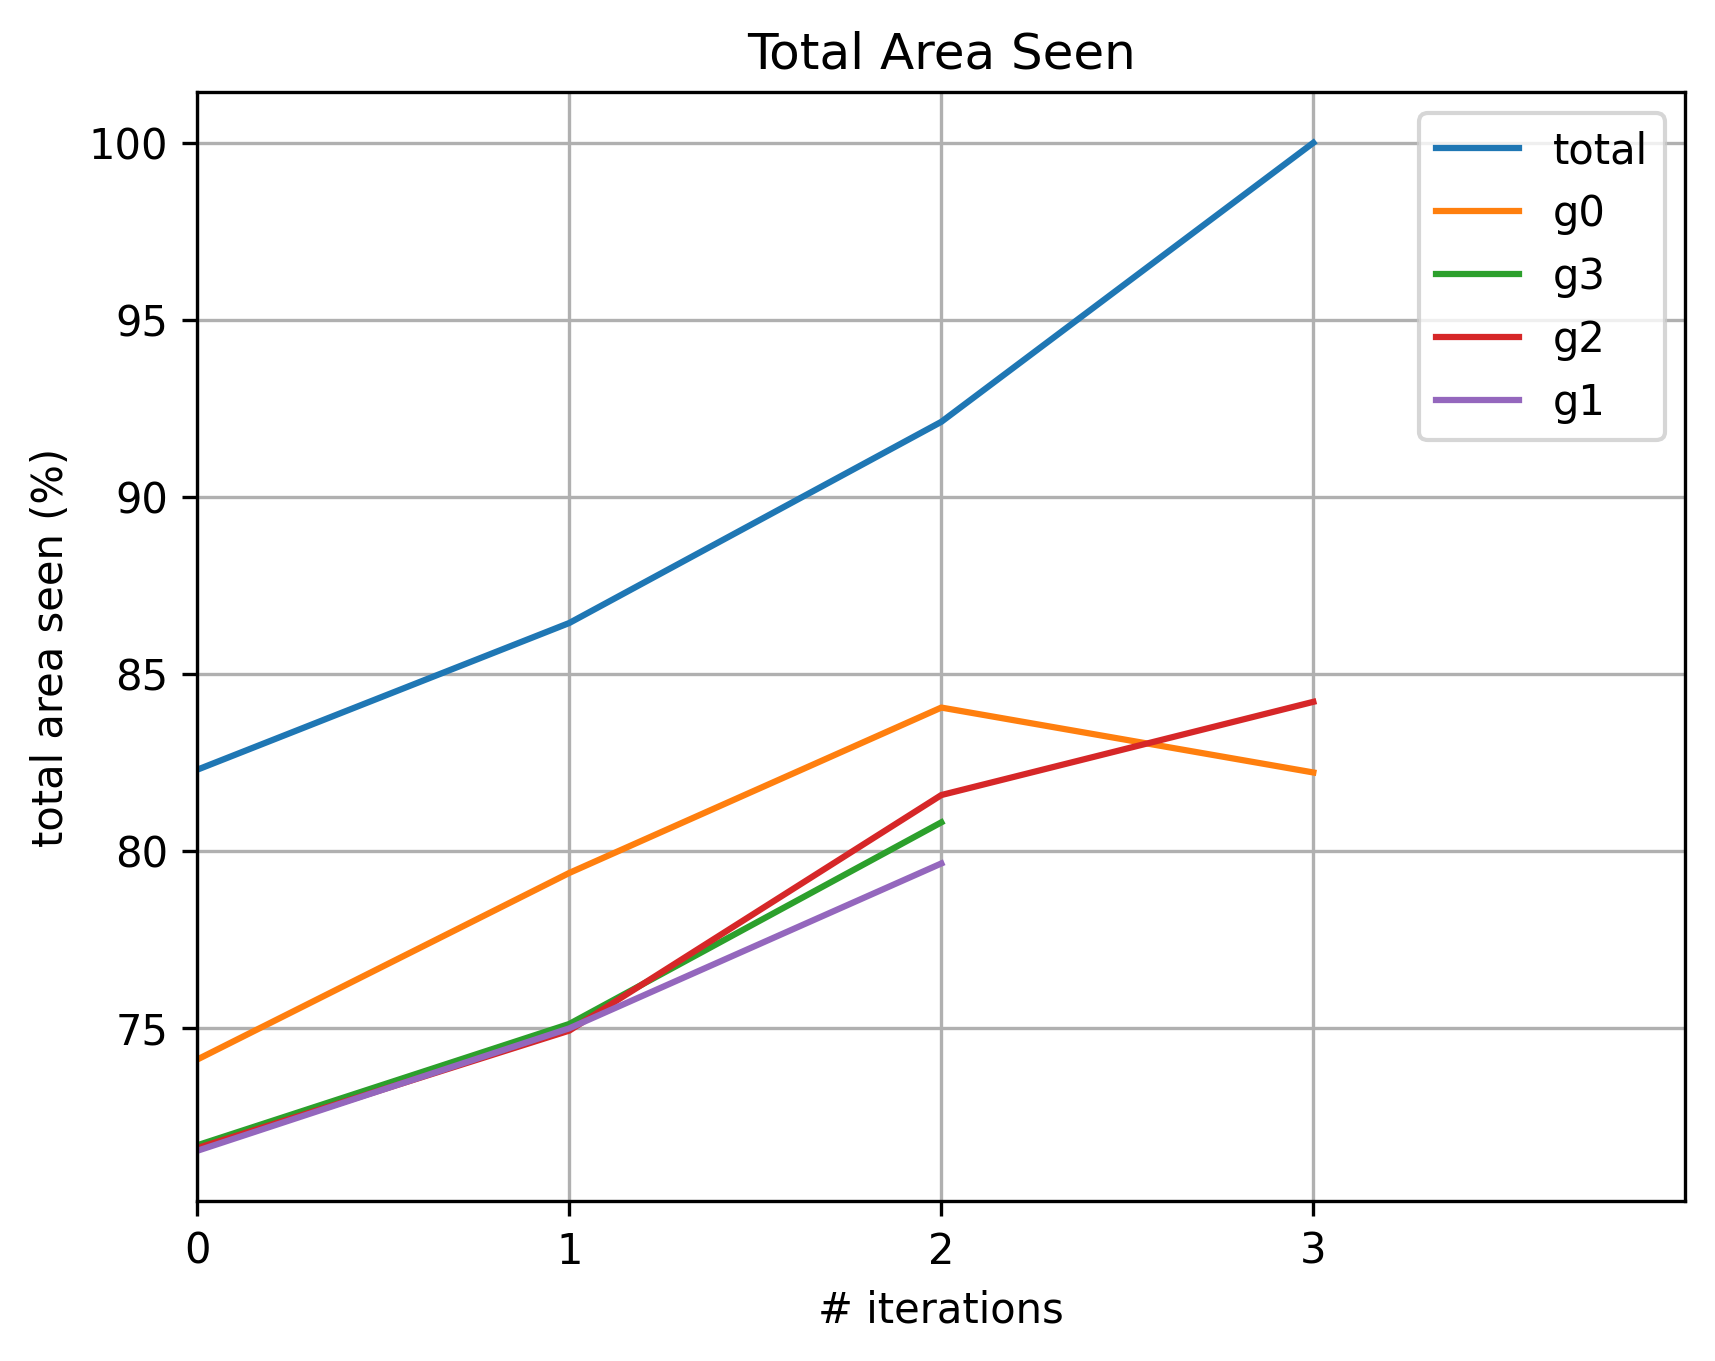
\includegraphics[width = \textwidth]{experiments/area_comb_easy_all.png}
        \caption{All heuristics.}
        \label{fig:no_line_search1}
    \end{subfigure}
    \begin{subfigure}{0.45\textwidth}
        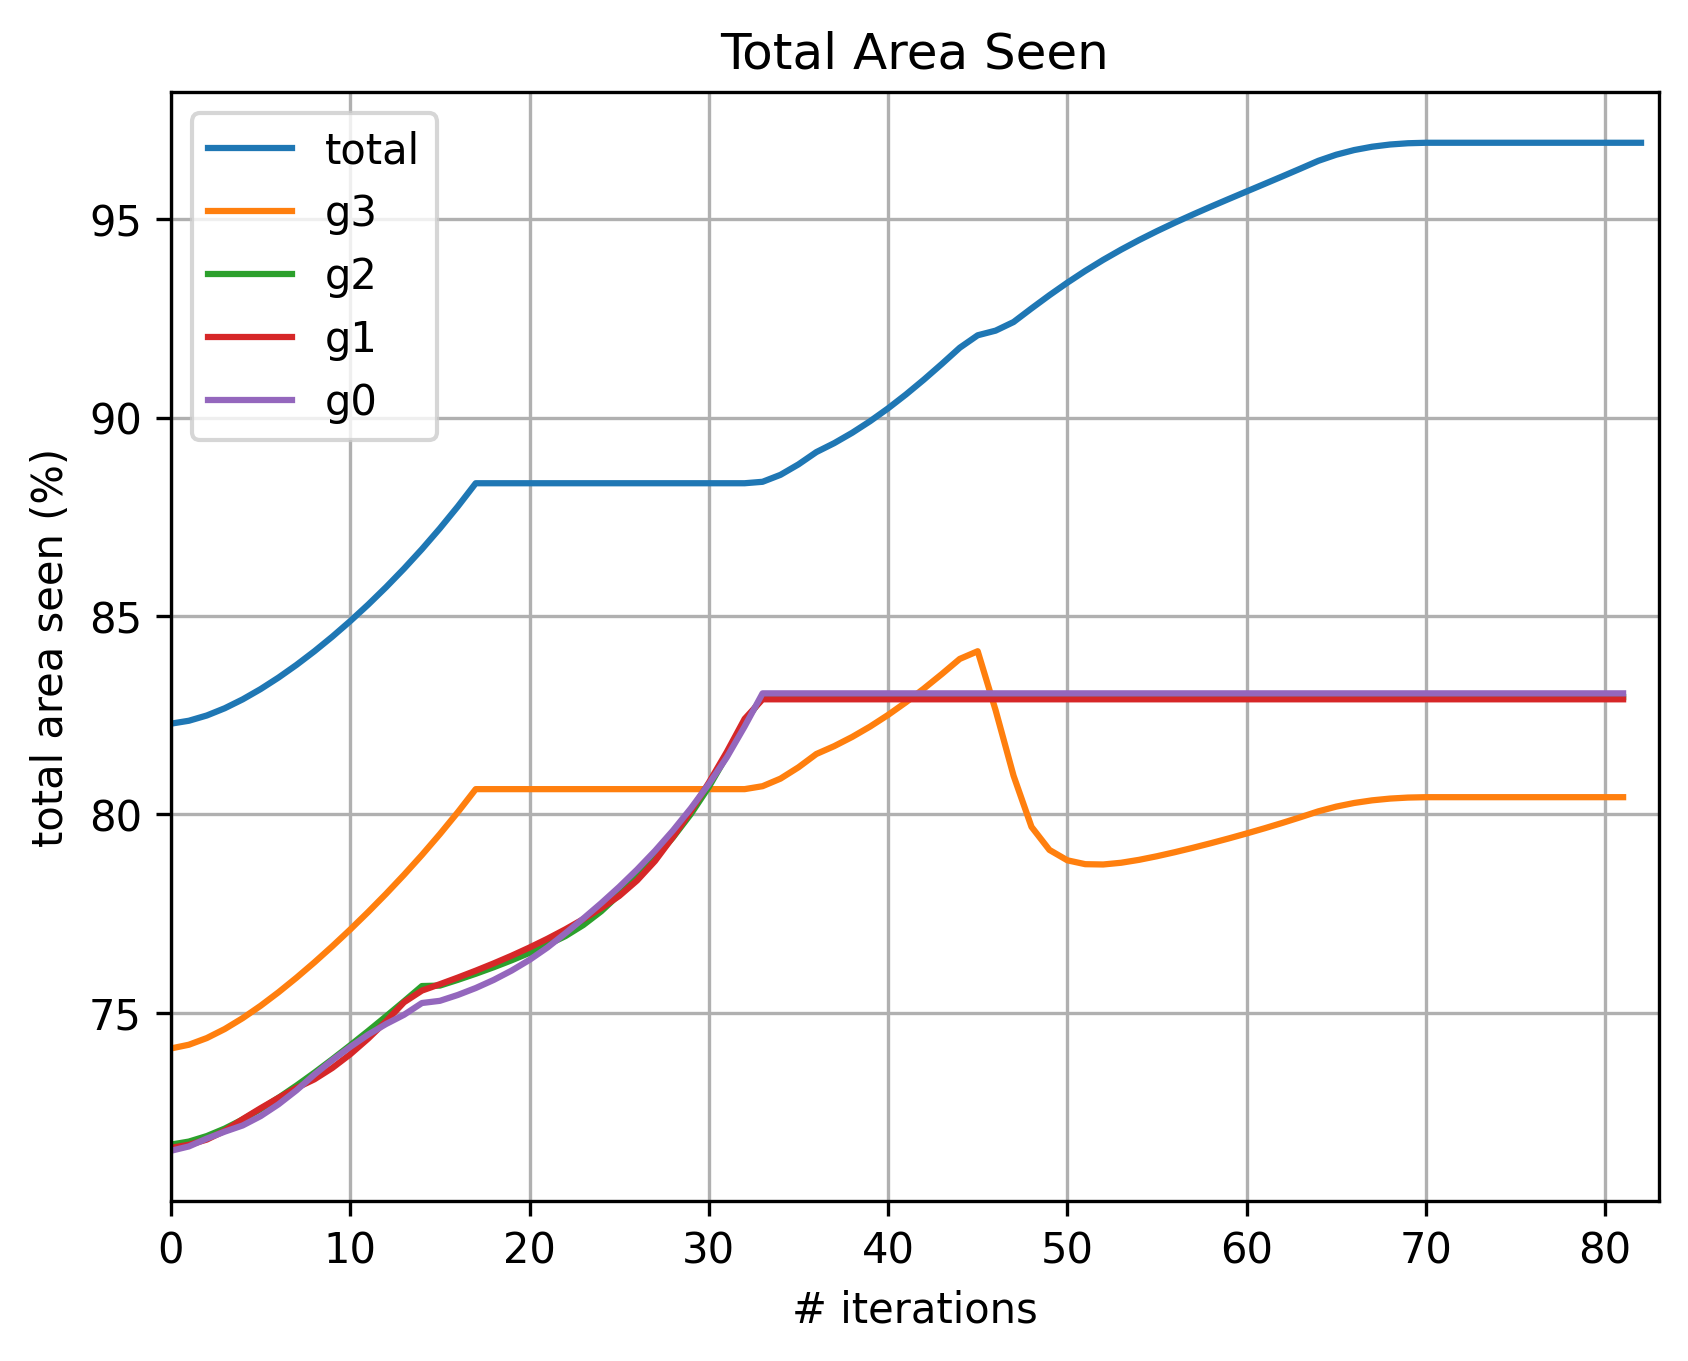
\includegraphics[width = \textwidth]{experiments/area_comb_no_linear_search.png}
        \caption{No line search.}
        \label{fig:no_line_search2}
    \end{subfigure}
    \caption{Total area seen per iteration for the comb polygon with four teeth.}
    \label{fig:no_line_search}
\end{figure}

\subsubsection{Without Pulling Onto Reflex Vertex}
In this section we will discuss the impact the pull onto the reflex vertex heuristic has on the behaviour of the algorithm. Section \ref{sec:pull_onto} introduced the pulling guards on top of a reflex vertex heuristic. This heuristic tackles the idea that if a guard is ``close enough'' to a reflex vertex, then the locally maximum seen area would be achieved by placing the guard on top of the reflex vertex. We have defined a guard being ``close enough'' to a reflex vertex as closer than two thirds of the minimum distance between any two reflex vertices in the polygon.

We will compare how the guards move when we are using all the heuristics to when we are not pulling them onto reflex vertices. The guards have a learning rate $\alpha = 0.4$ and start at the same fixed position in both cases.

Figure \ref{fig:no_pull} displays the two reflex vertex pull cases: Subfigures \ref{fig:all_pull_pos0} and \ref{fig:all_pull_pos1} show how the green guard movement changes when it is placed onto the reflex vertex; Subfigures \ref{fig:no_pull_pos0} and \ref{fig:no_pull_pos1} show how the guard movement changes when the guard is pulled towards the reflex vertex, but not pulled onto it. We can observe how in Subfigure \ref{fig:all_pull_pos1} the green guard is placed onto the reflex vertex. It then strives to reach the unseen polygon part in the upper left corner. On the other hand, in Subfigure \ref{fig:no_pull_pos1} the guard moved away from the reflex vertex. However, its movement still indicates that it should move back, closer to the reflex vertex it was not placed on. 
This behaviour is also reflected in the two seen area plots in Subfigures \ref{fig:area_all_pull} and Subfigures \ref{fig:area_no_pull}. Clearly, the case when the green guard is not placed on top of the reflex vertex results in more iterations, as seen in Subfigure \ref{fig:area_no_pull}. This is due to the fact that the green guard could not take advantage of the local area maximisation by being placed on the reflex vertex. So, it needs to move around more before finding its optimal path. This is also displayed in how the total area seen stagnates in between iterations 2 and 4. Conversely, Subfigure \ref{fig:area_all_pull} displays how the green guard has quickly moved towards the last part of the polygon that was not yet seen. This resulted in a steady increase in the total seen area.

Therefore, we believe that pulling guards on top of reflex vertices when they are ``close enough'' results in the local maximisation of the area seen by those guards. The number of iterations needed to reach the global maximum is thus reduced. So, the efficiency of the algorithm is also positively affected.

\begin{figure}[h!]
    \centering
    \begin{subfigure}{0.45\textwidth}
        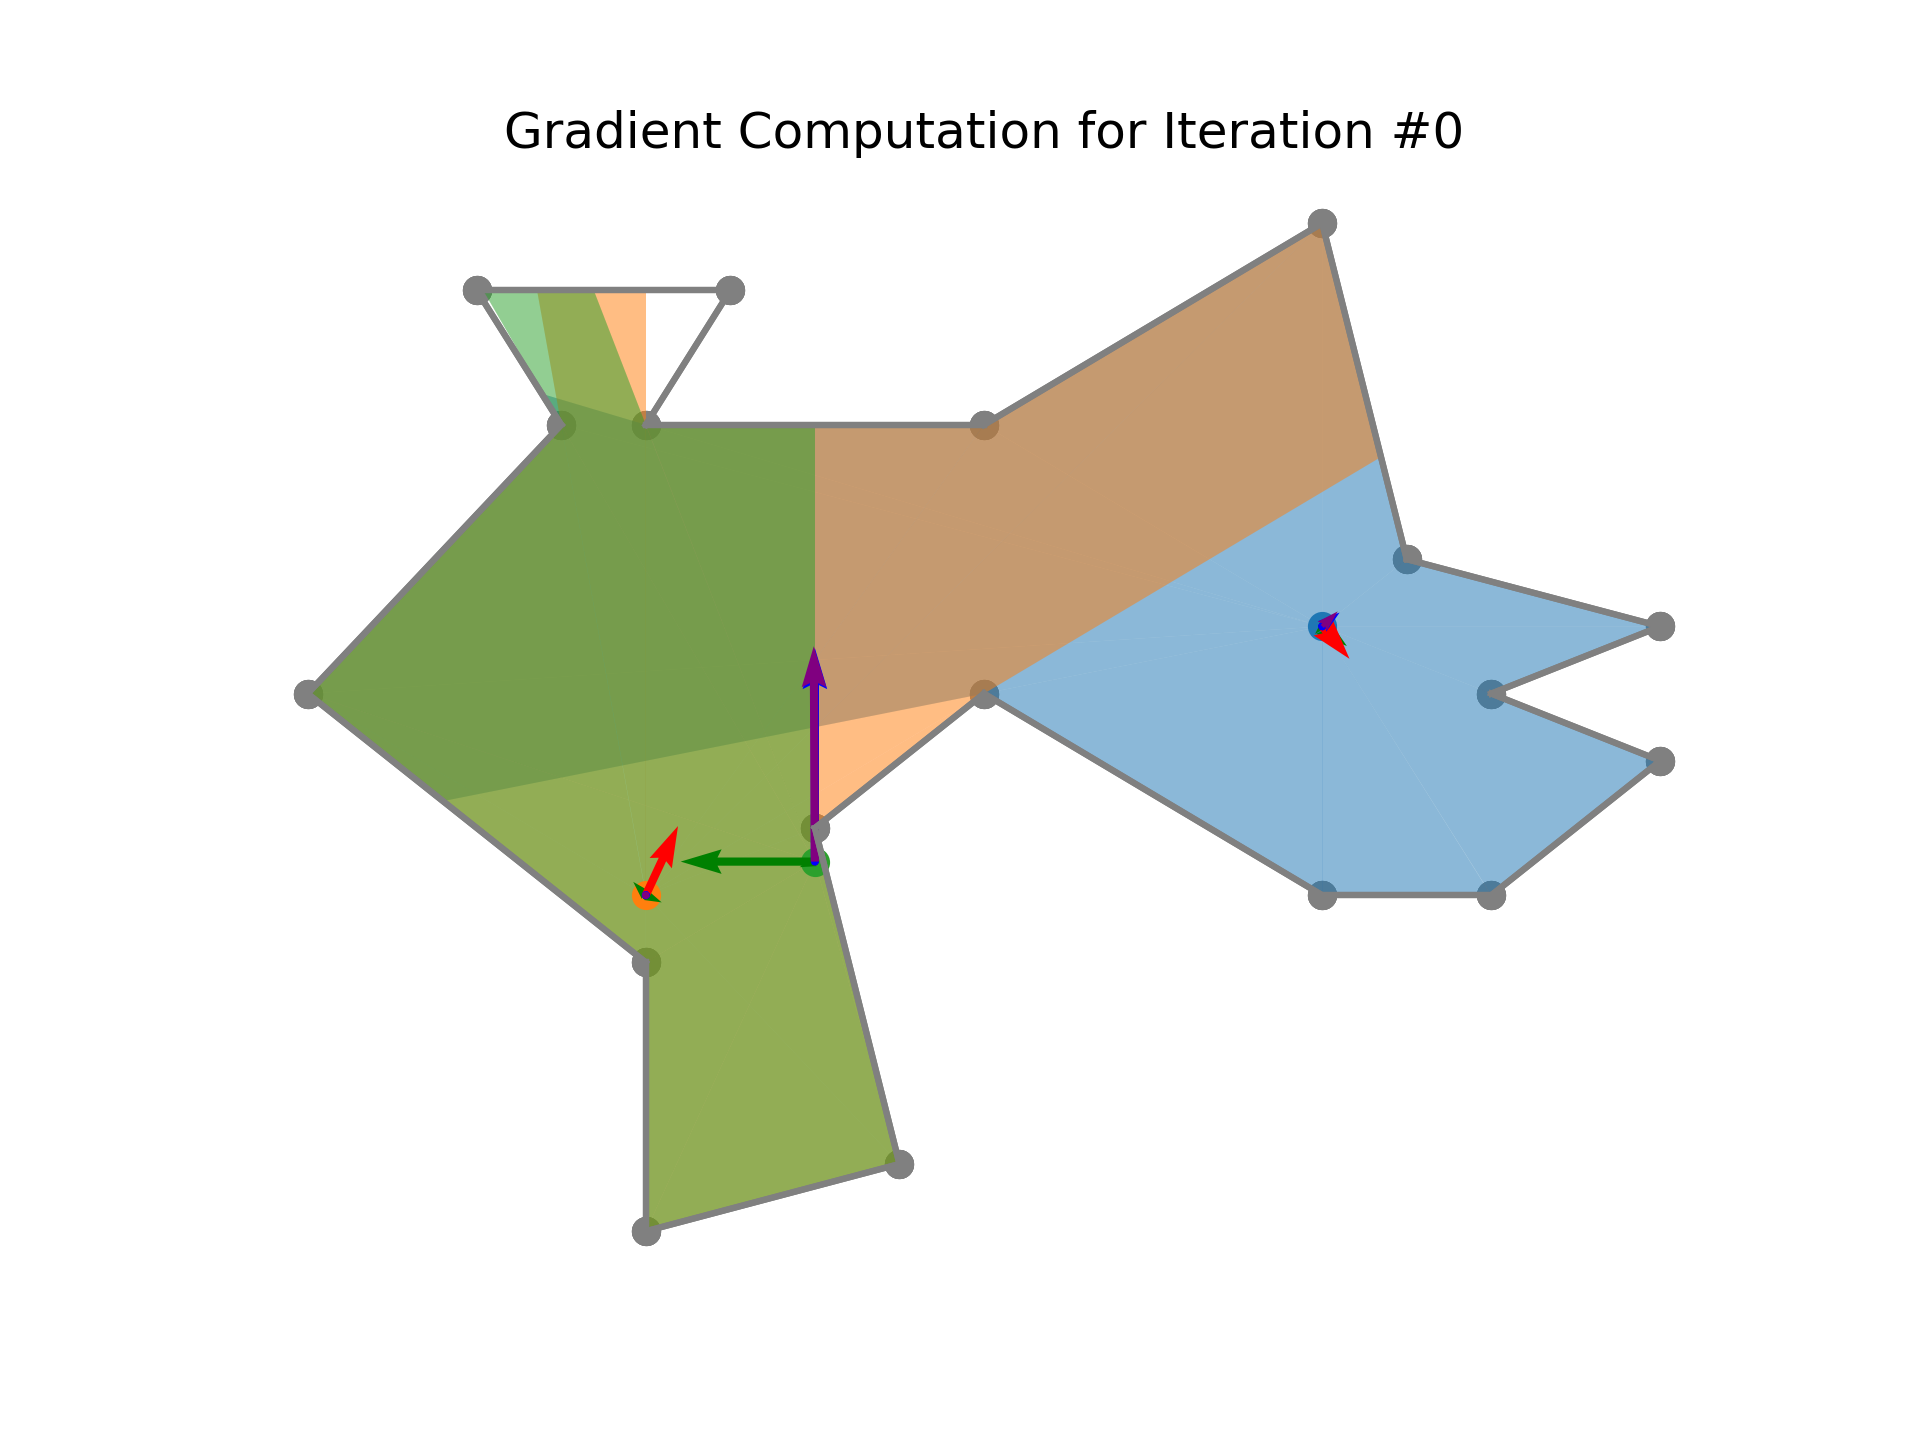
\includegraphics[width = \textwidth]{experiments/random_all_pull_pos0.png}
        \caption{All heuristics, iteration 0. The guard is pulled towards the reflex vertex.}
        \label{fig:all_pull_pos0}
    \end{subfigure}
    \hfill
    \begin{subfigure}{0.45\textwidth}
        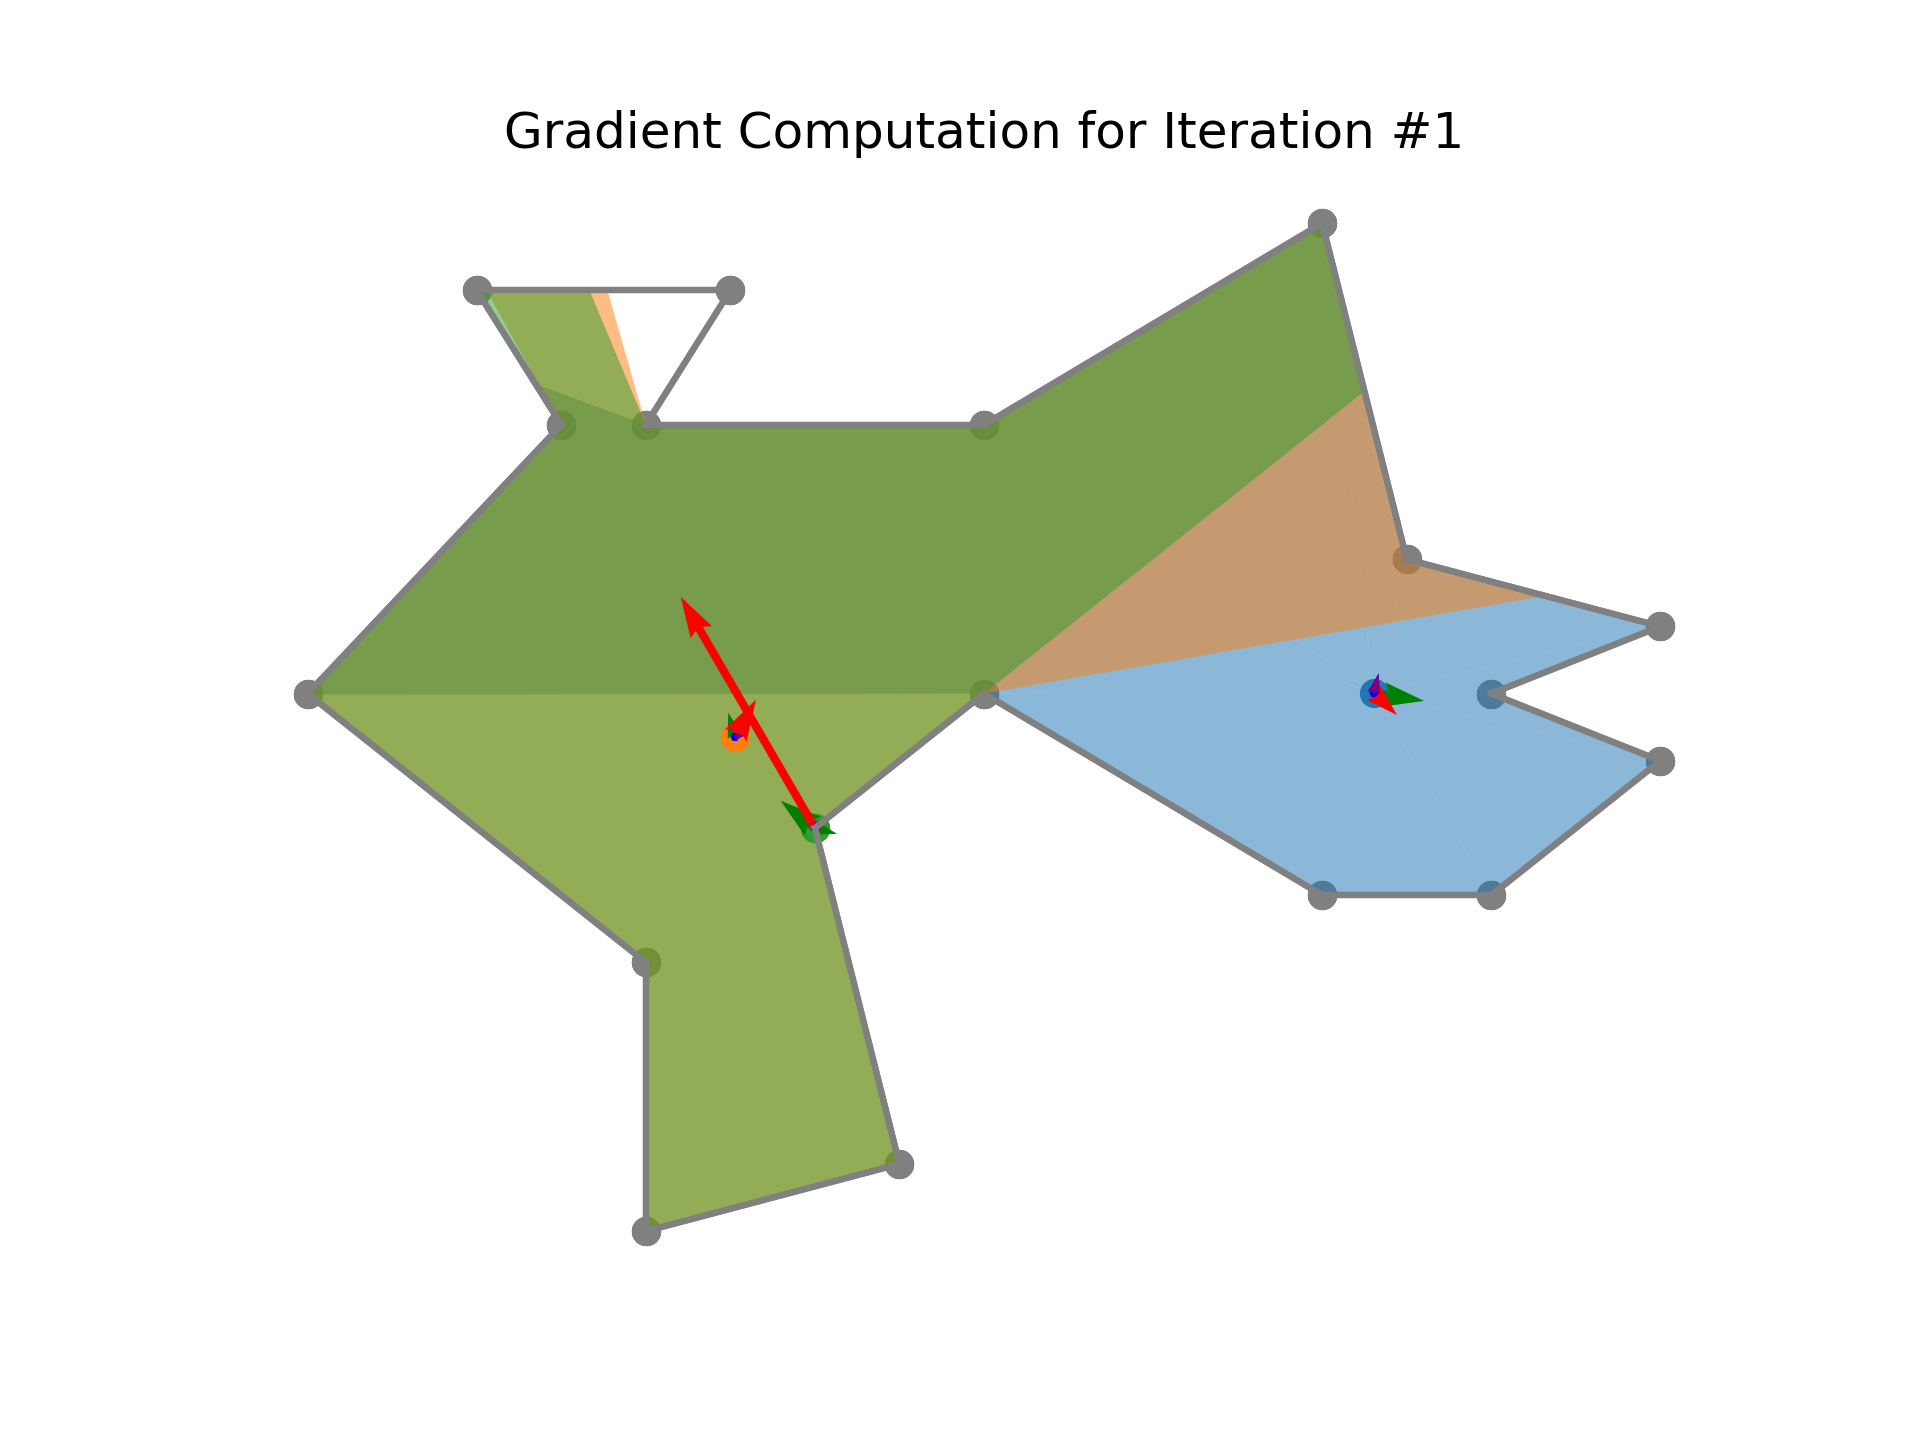
\includegraphics[width = \textwidth]{experiments/random_all_pull_pos1.png}
        \caption{All heuristics, iteration 1. The guard is onto the reflex vertex.}
        \label{fig:all_pull_pos1}
    \end{subfigure}
    \vfill
    \begin{subfigure}{0.45\textwidth}
        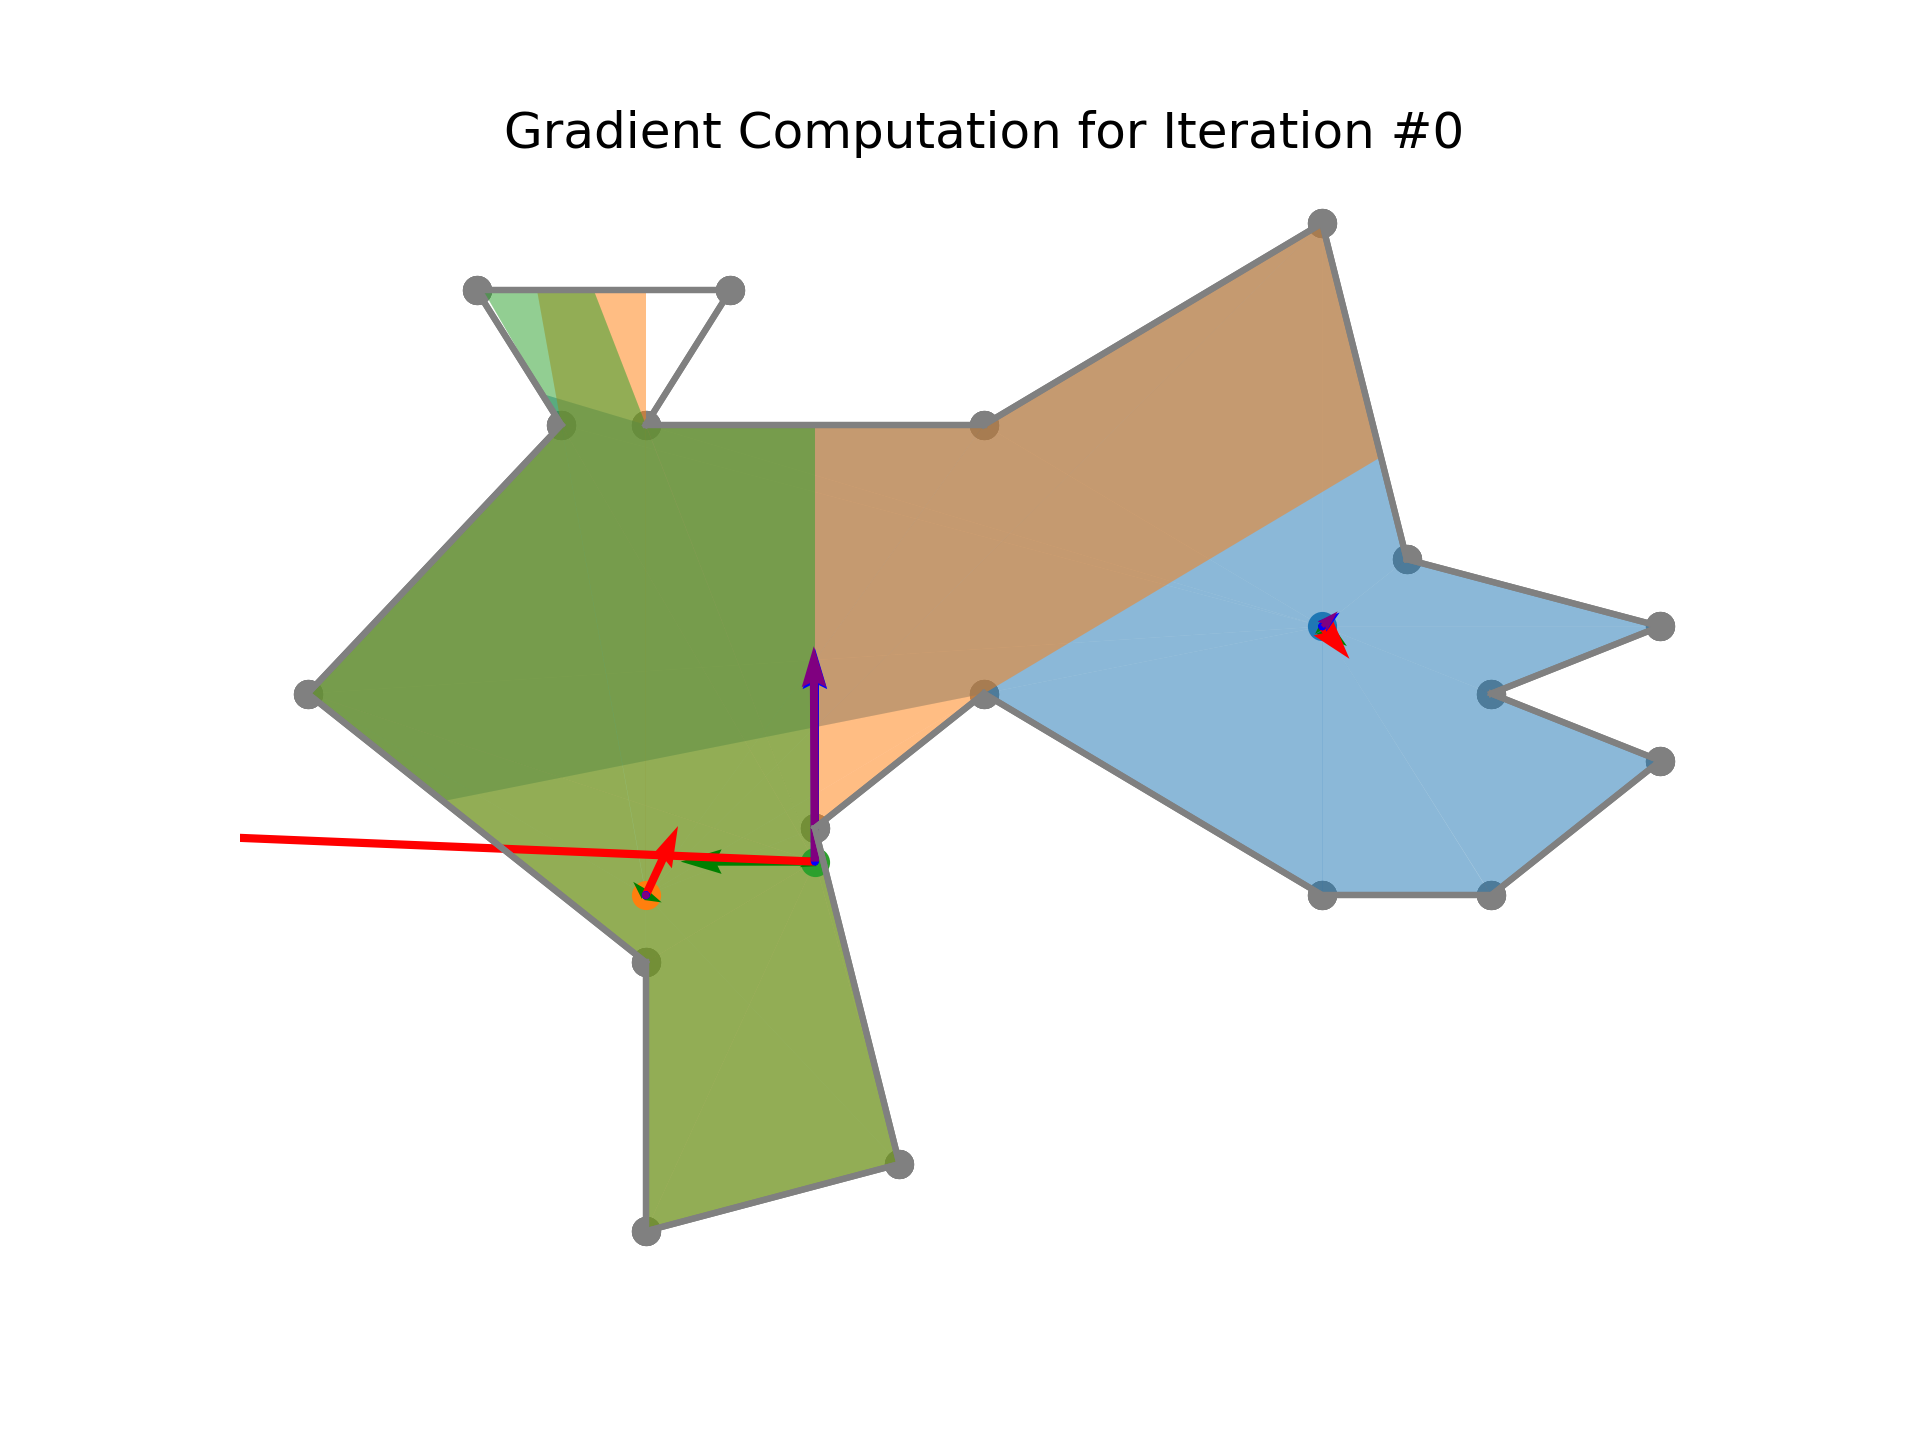
\includegraphics[width = \textwidth]{experiments/random_no_pull_pos0.png}
        \caption{No pull onto the reflex vertex, iteration 0. The guard is pulled towards the reflex vertex.}
        \label{fig:no_pull_pos0}
    \end{subfigure}
    \hfill
    \begin{subfigure}{0.45\textwidth}
        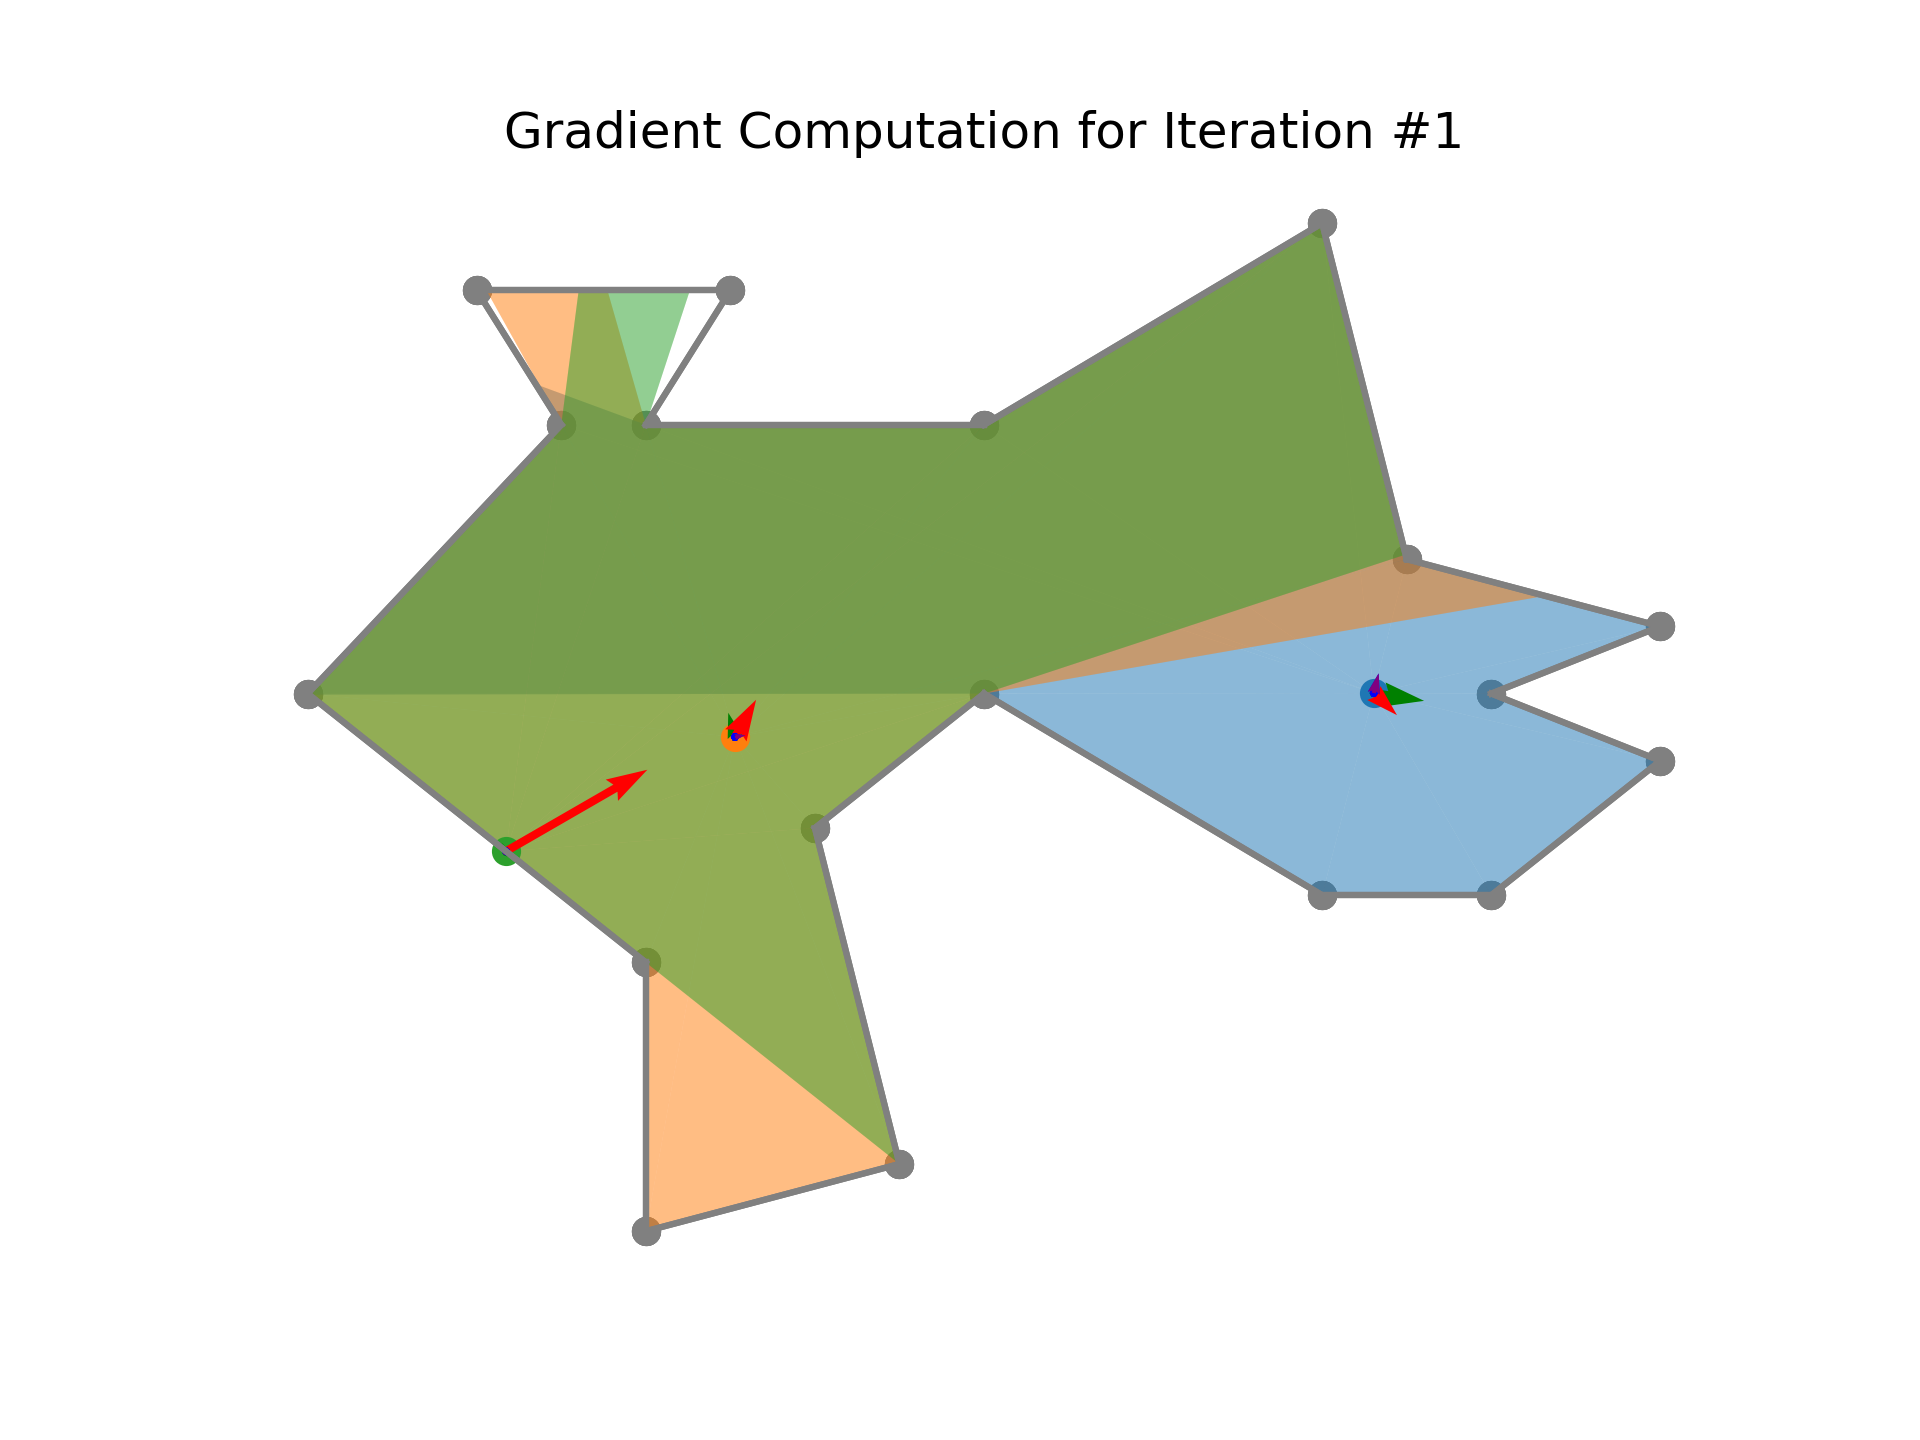
\includegraphics[width = \textwidth]{experiments/random_no_pull_pos1.png}
        \caption{No pull onto the reflex vertex, iteration 1. The guard is placed according to the momentum computation.}
        \label{fig:no_pull_pos1}
    \end{subfigure}
    \vfill
    \begin{subfigure}{0.45\textwidth}
        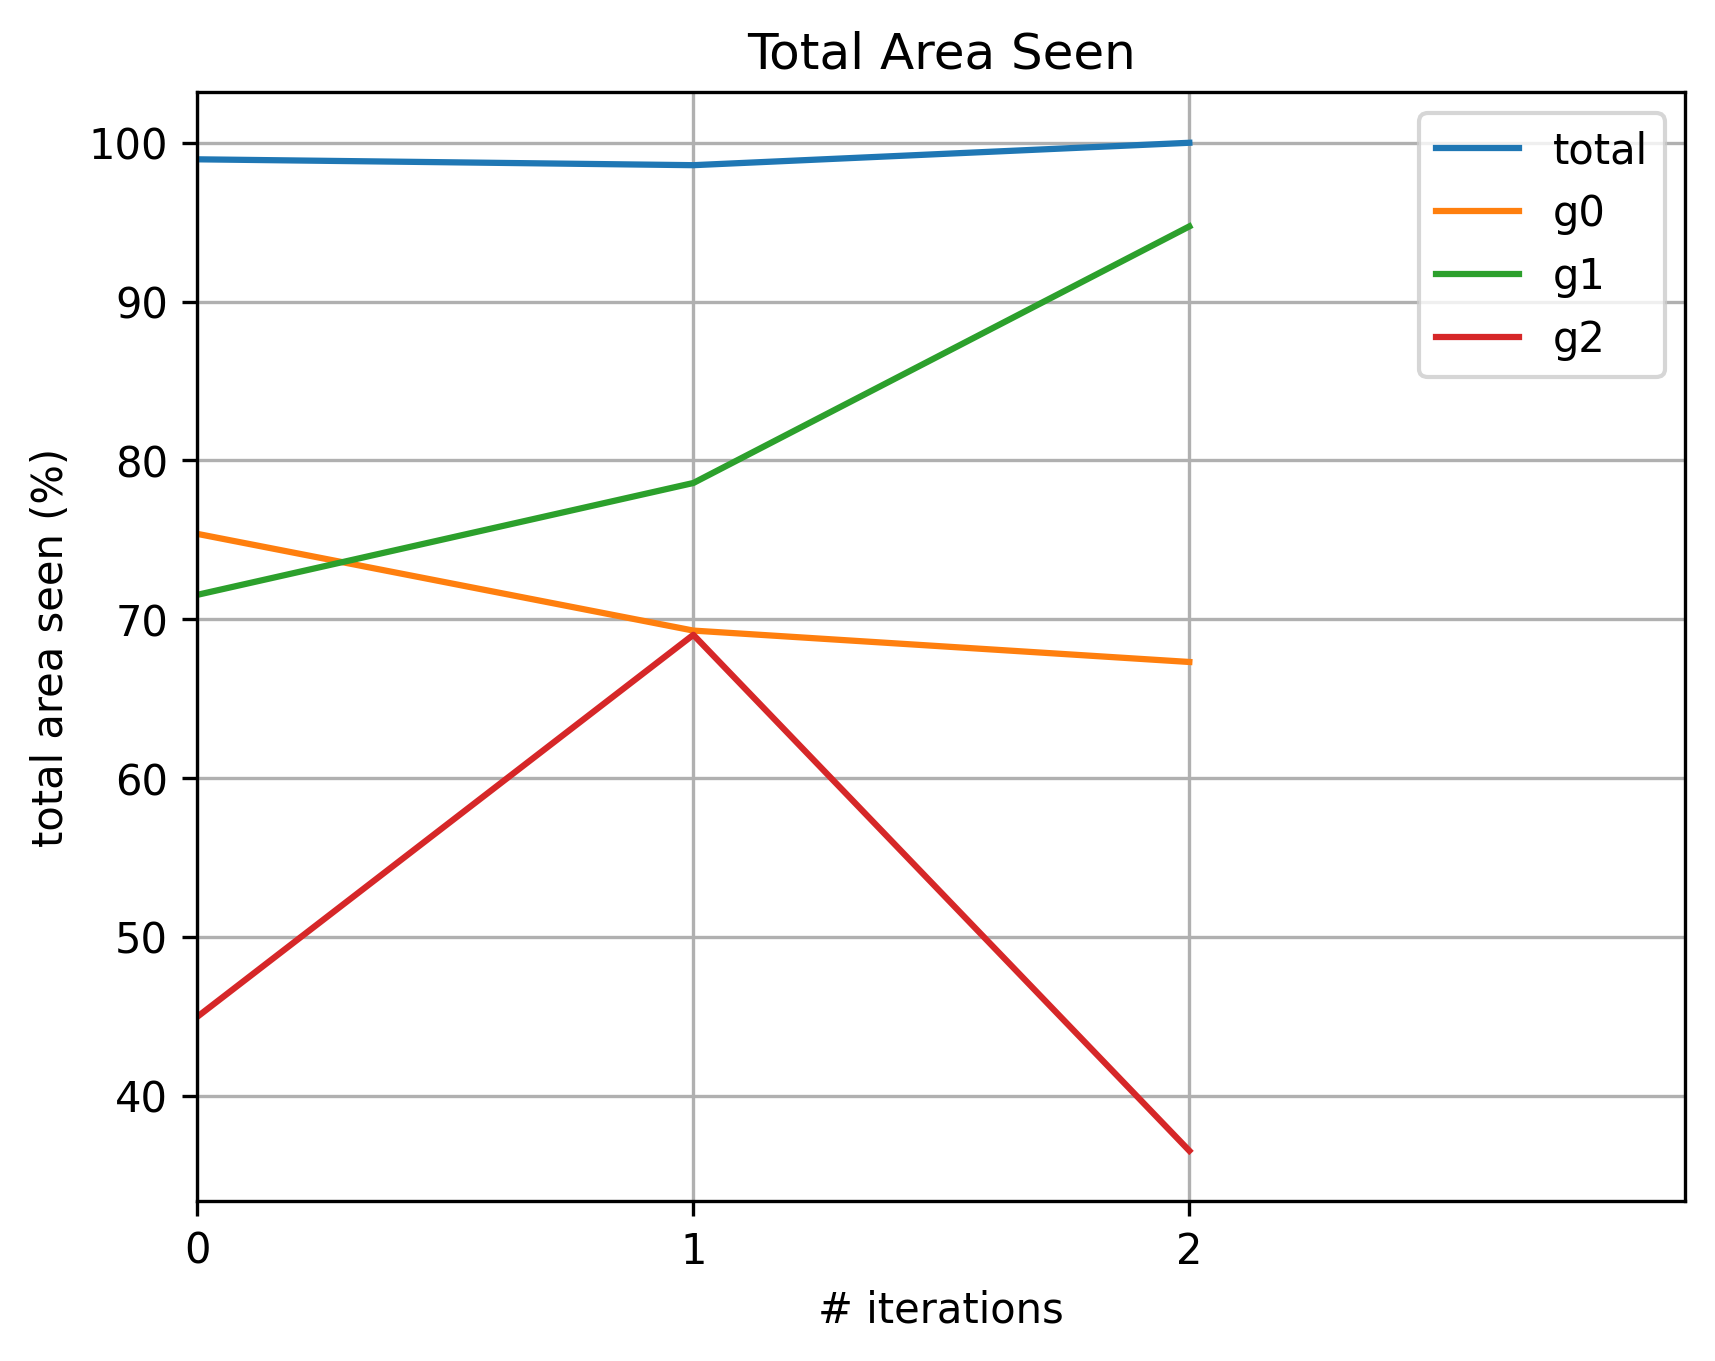
\includegraphics[width = \textwidth]{experiments/area_random_all_pull_onto.png}
        \caption{Seen area for all heuristics.}
        \label{fig:area_all_pull}
    \end{subfigure}
    \hfill
    \begin{subfigure}{0.45\textwidth}
        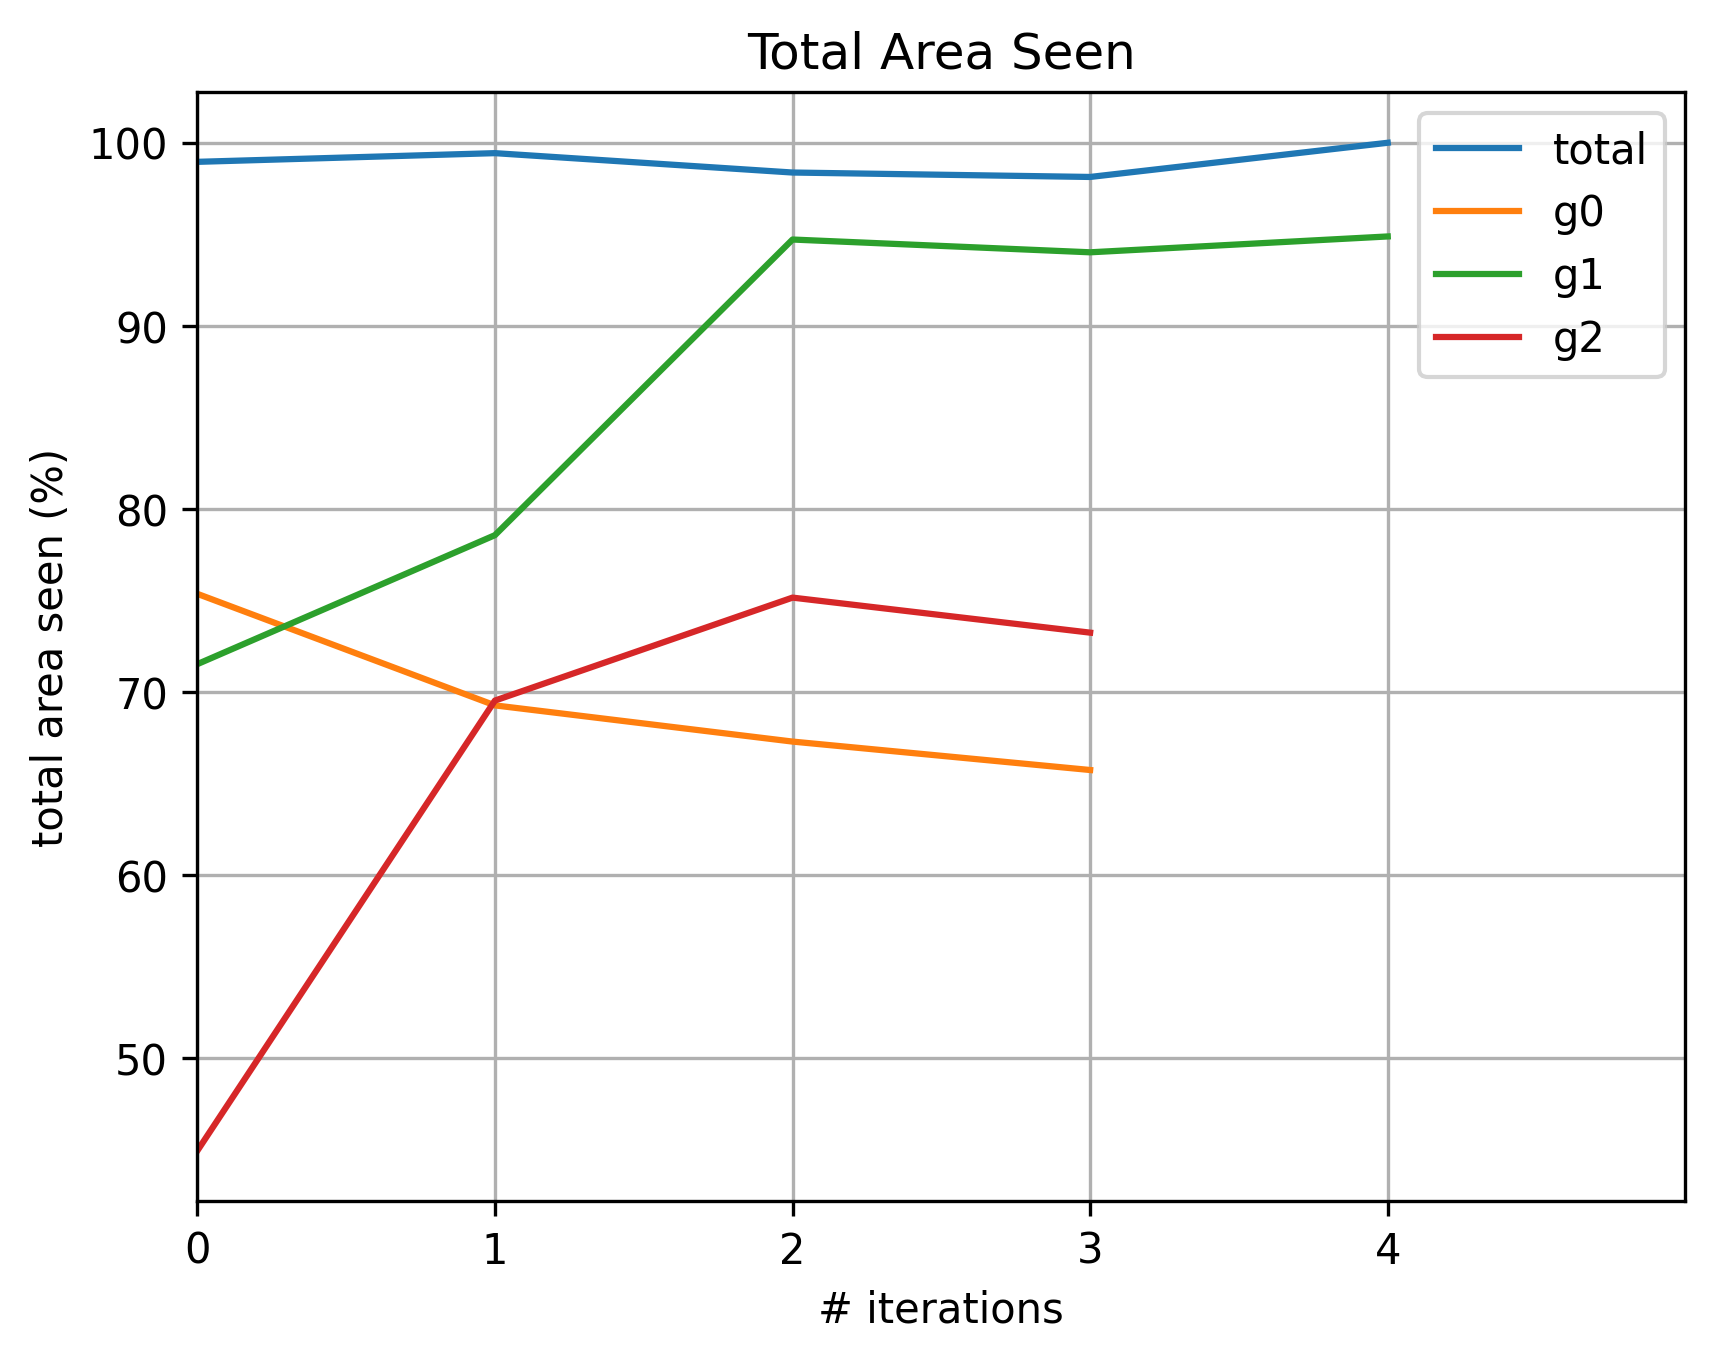
\includegraphics[width = \textwidth]{experiments/area_random_no_pull_onto.png}
        \caption{Seen area without pull onto reflex vertices.}
        \label{fig:area_no_pull}
    \end{subfigure}
    \caption{Example of a guard being pulled towards a reflex vertex in the arbitrary polygon.}
    \label{fig:no_pull}
\end{figure}

\subsubsection{Without Pull Capping}
In this section we will discuss how not capping the pull towards a reflex vertex influences the overall progression of the guards' movements. Section \ref{sec:pull_capping} introduced the notion of capping the pull towards a reflex vertex. The reason for this choice was to not give the pull the possibility to overpower the value of the momentum. So, if the pull is larger than a factor $\mu$ than the momentum, it is capped at the momentum value of a factor of $\mu$. 

We will compare how the guards move when we are using all the heuristics to when we are not capping the pull towards reflex vertices. We will use the comb polygon with four teeth as example. The guards have a learning rate $\alpha = 0.4$ and a pull cap hyperparameter $\mu = 1$. Thus, if the pull is larger than the momentum, we cap it at the size of the momentum. The reason behind this hyperparameter choice was that it offers a middle ground in between pull capping values that are significantly larger or smaller than the momentum. So, if the pull is as large as the momentum, we will decide to prioritise giving the guard the choice to be pulled onto a reflex vertex if it is ``close enough''.

Figure \ref{fig:no_capping} displays the two reflex vertex pull cases: Subfigures \ref{fig:all_cap_pos0} and \ref{fig:all_cap_pos1} show how the blue guard movement changes when its pull is capped; Subfigures \ref{fig:no_cap_pos0} and \ref{fig:no_cap_pos1} show the opposite. We can observe how in Subfigure \ref{fig:all_cap_pos0} the blue guard has its pull towards the reflex vertex capped. In that case, the pull is not strong enough to move the guard towards the reflex vertex. So, the blue guard moves as its momentum dictates to the position in Subfigure \ref{fig:all_cap_pos1}. This can result in encouraging the guard to explore the polygon more rather than directly moving towards a reflex vertex.
Conversely, Subfigure \ref{fig:no_cap_pos1} displays the blue guard moving closer to the reflex vertex it is pulled to. In subsequent iterations, it is placed on the reflex vertex

Subfigures \ref{fig:area_all_cap} and \ref{fig:area_no_cap} show how the global behaviour of the algorithm is influenced by the capping. Interestingly enough, when capping the pull, the guards' behaviour is more erratic, resulting in more iterations before the whole polygon is seen. On the other hand, using no capping allows a steadier increase in the total area seen. Eventually, the blue guard is drawn and placed onto the reflex vertex. This reinforces the previously discussed idea that placing guards on reflex vertices is beneficial for the overall run of the algorithm. Nonetheless, tuning the hyperparameter $\mu$ is a crucial point of exploration for deciding how and when pull capping would always prove most beneficial.

Therefore, we believe that capping the guards' pull towards a reflex vertex highly depends on the hyperparameter $\mu$ and the shape of the polygon. When not capped, it additionally reinforces the importance of placing guards on reflex vertices. However, when the pull of guards is capped, we are using a more exploratory approach to discovering the polygon.

\begin{figure}[h!]
    \centering
    \begin{subfigure}{0.45\textwidth}
        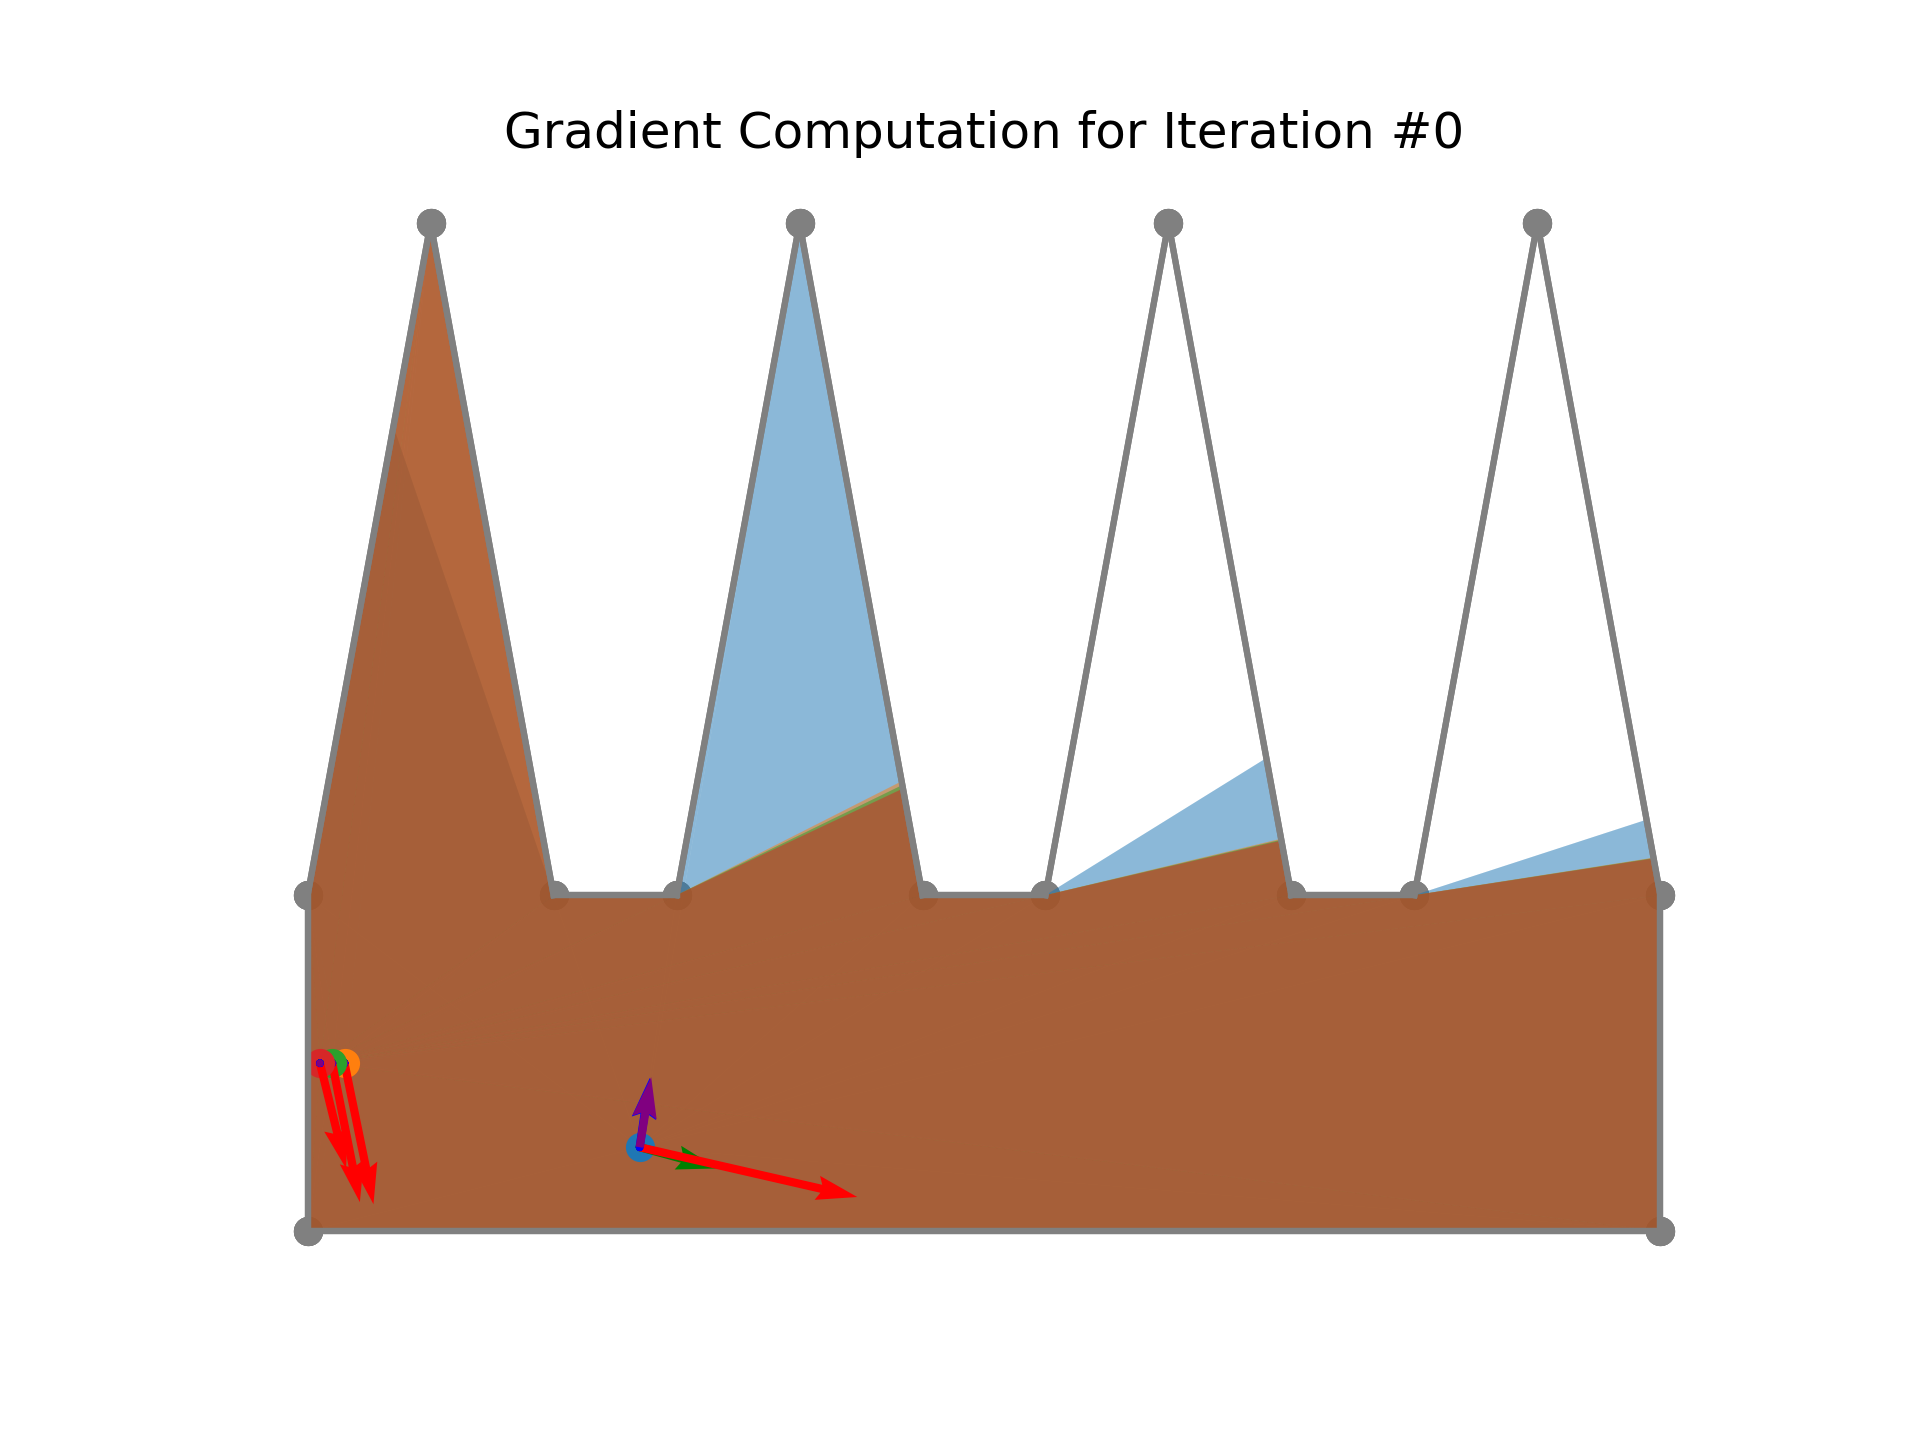
\includegraphics[width = \textwidth]{experiments/comb_capping_pos0.png}
        \caption{All heuristics, iteration 0. The guard's pull towards the reflex vertex is capped.}
        \label{fig:all_cap_pos0}
    \end{subfigure}
    \hfill
    \begin{subfigure}{0.45\textwidth}
        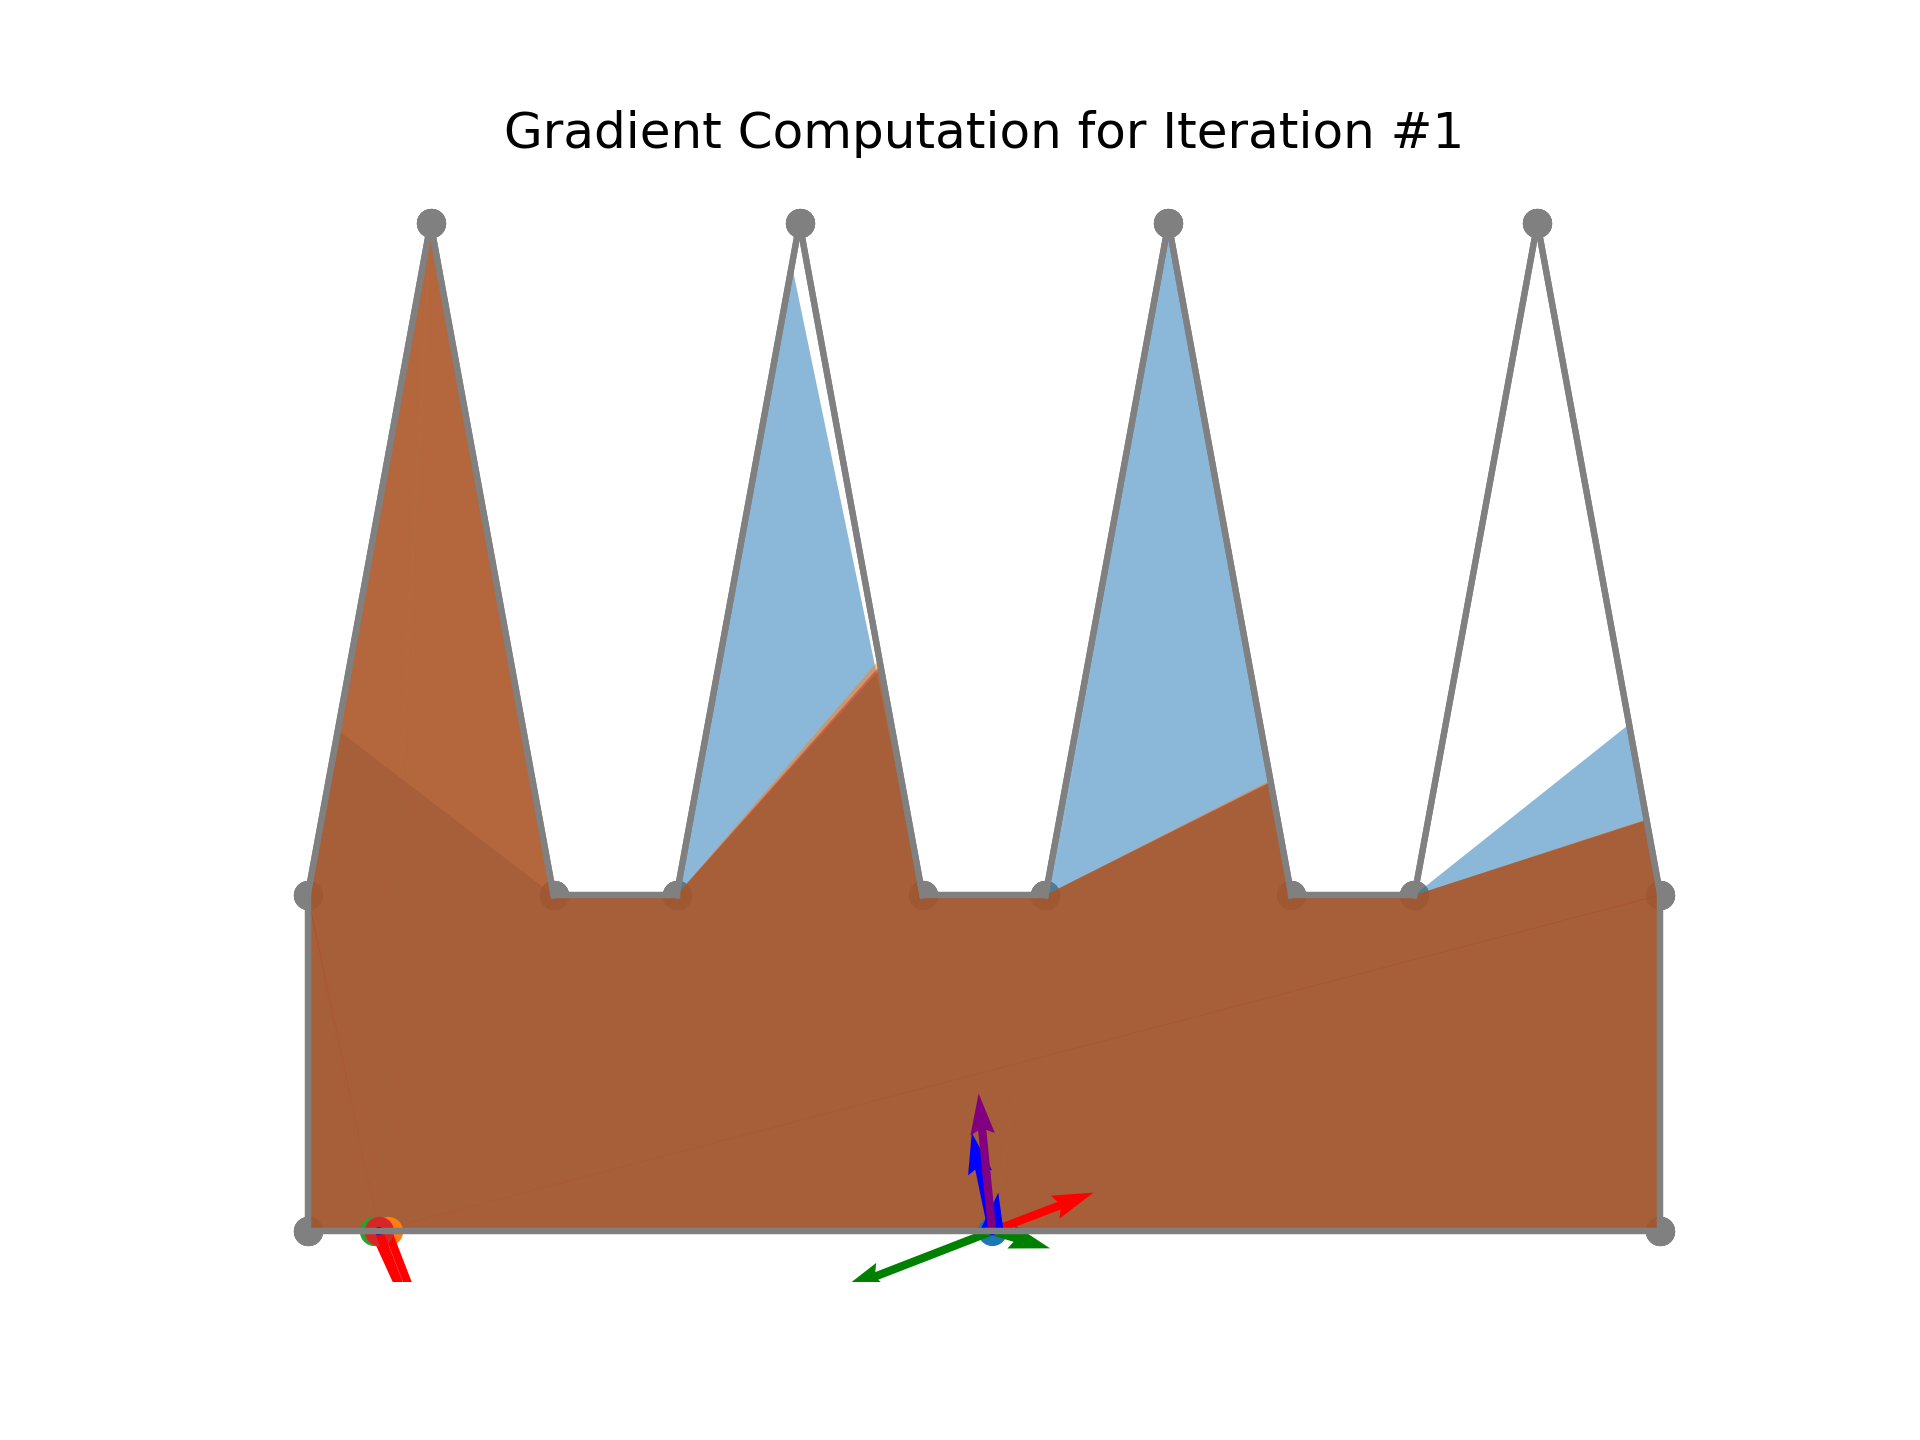
\includegraphics[width = \textwidth]{experiments/comb_capping_pos1.png}
        \caption{All heuristics, iteration 1. The guard does not act upon the pull towards the reflex vertex.}
        \label{fig:all_cap_pos1}
    \end{subfigure}
    \vfill
    \begin{subfigure}{0.45\textwidth}
        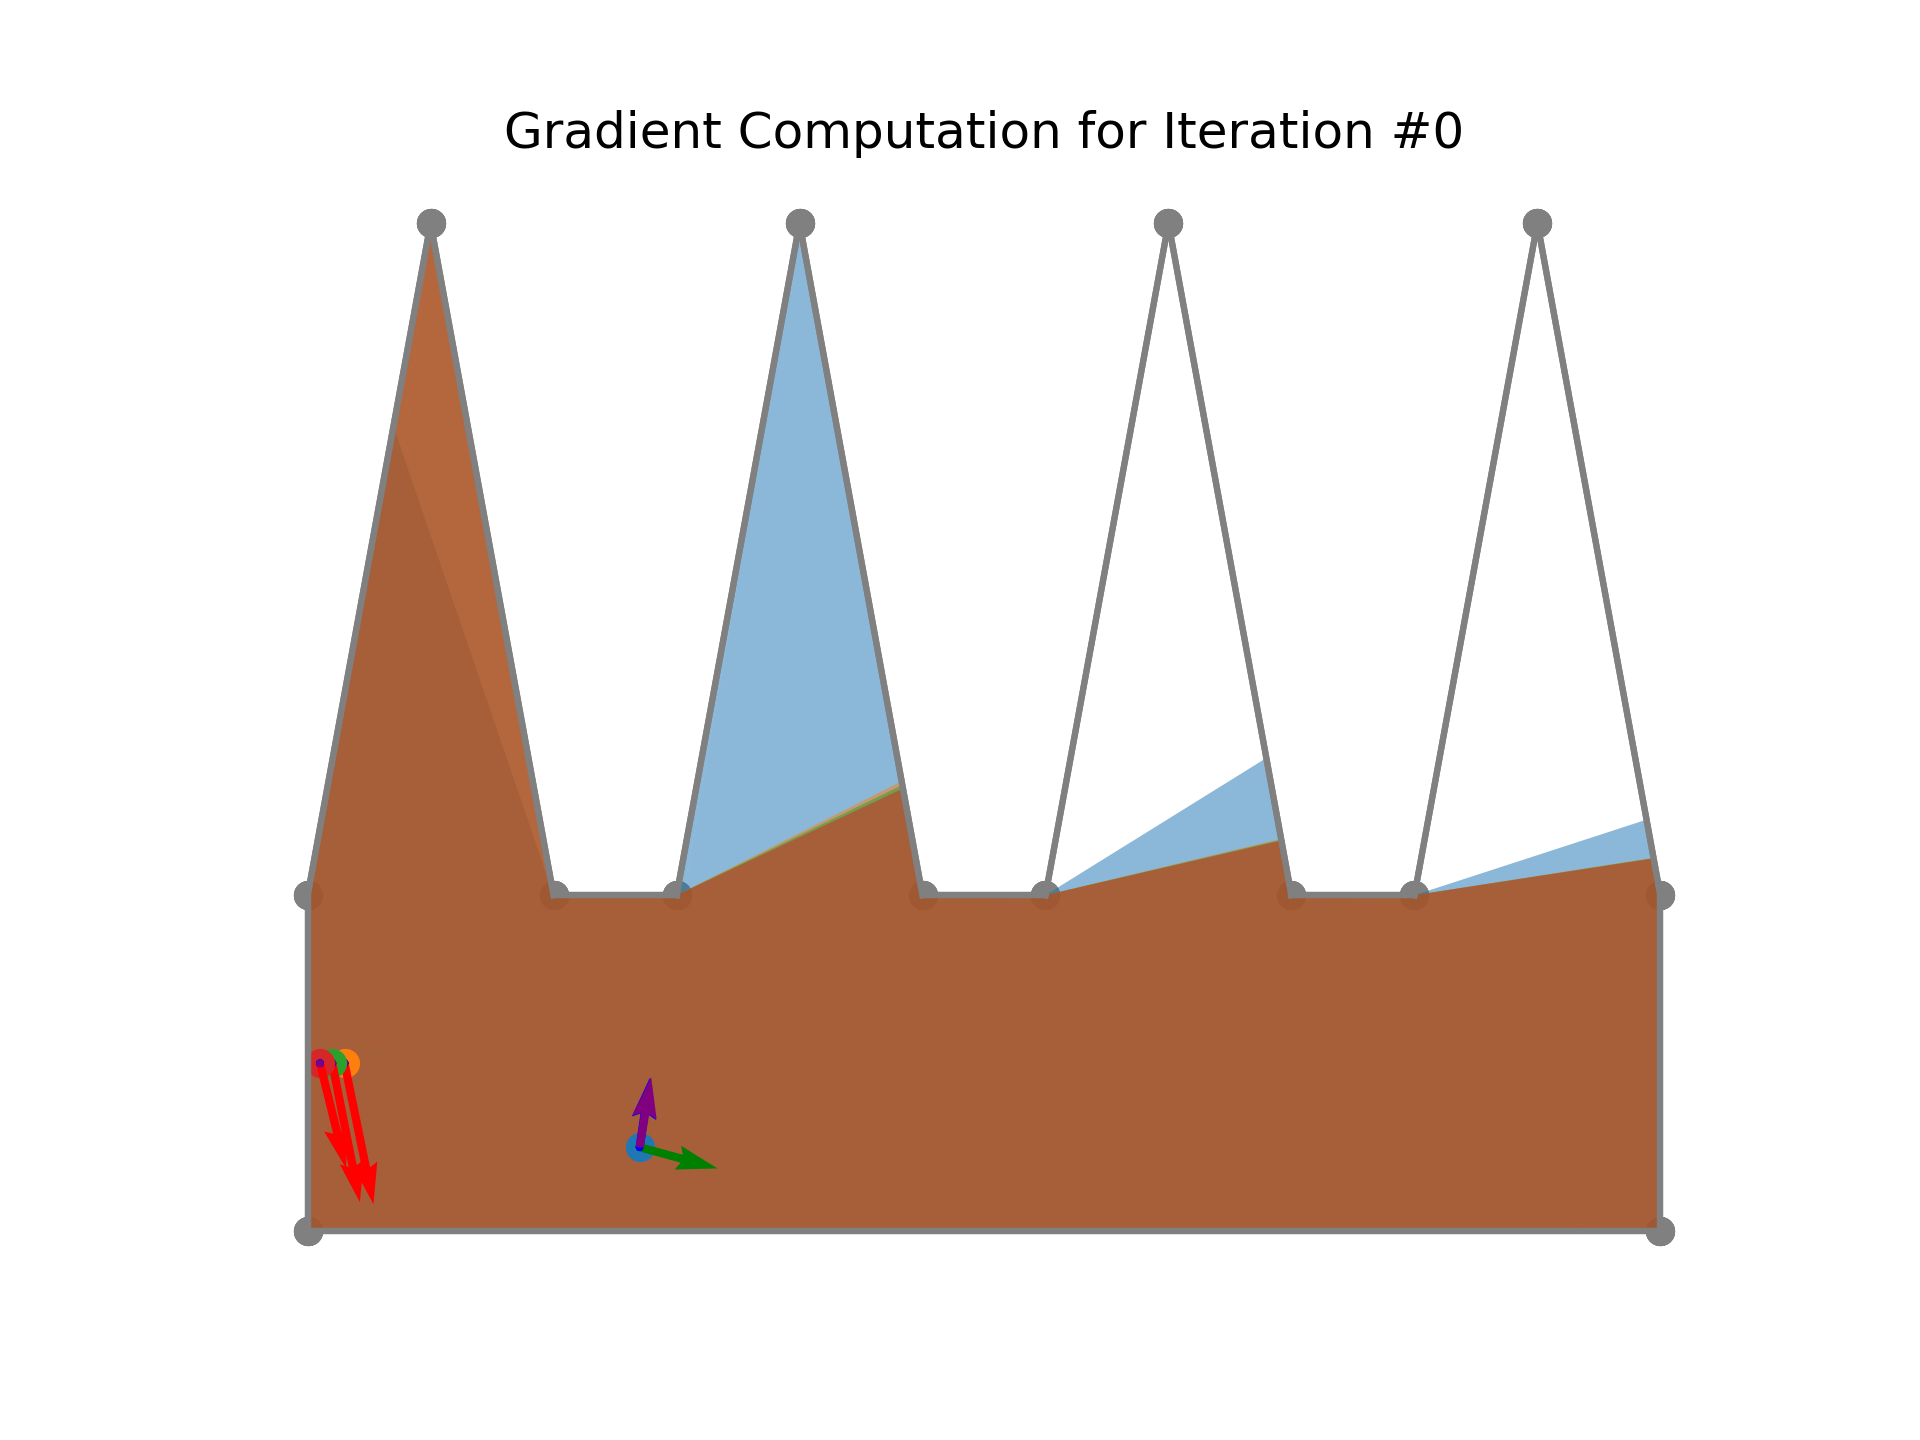
\includegraphics[width = \textwidth]{experiments/comb_no_capping_pos0.png}
        \caption{No pull onto the reflex vertex, iteration 0. The guard's pull towards the reflex vertex is not capped.}
        \label{fig:no_cap_pos0}
    \end{subfigure}
    \hfill
    \begin{subfigure}{0.45\textwidth}
        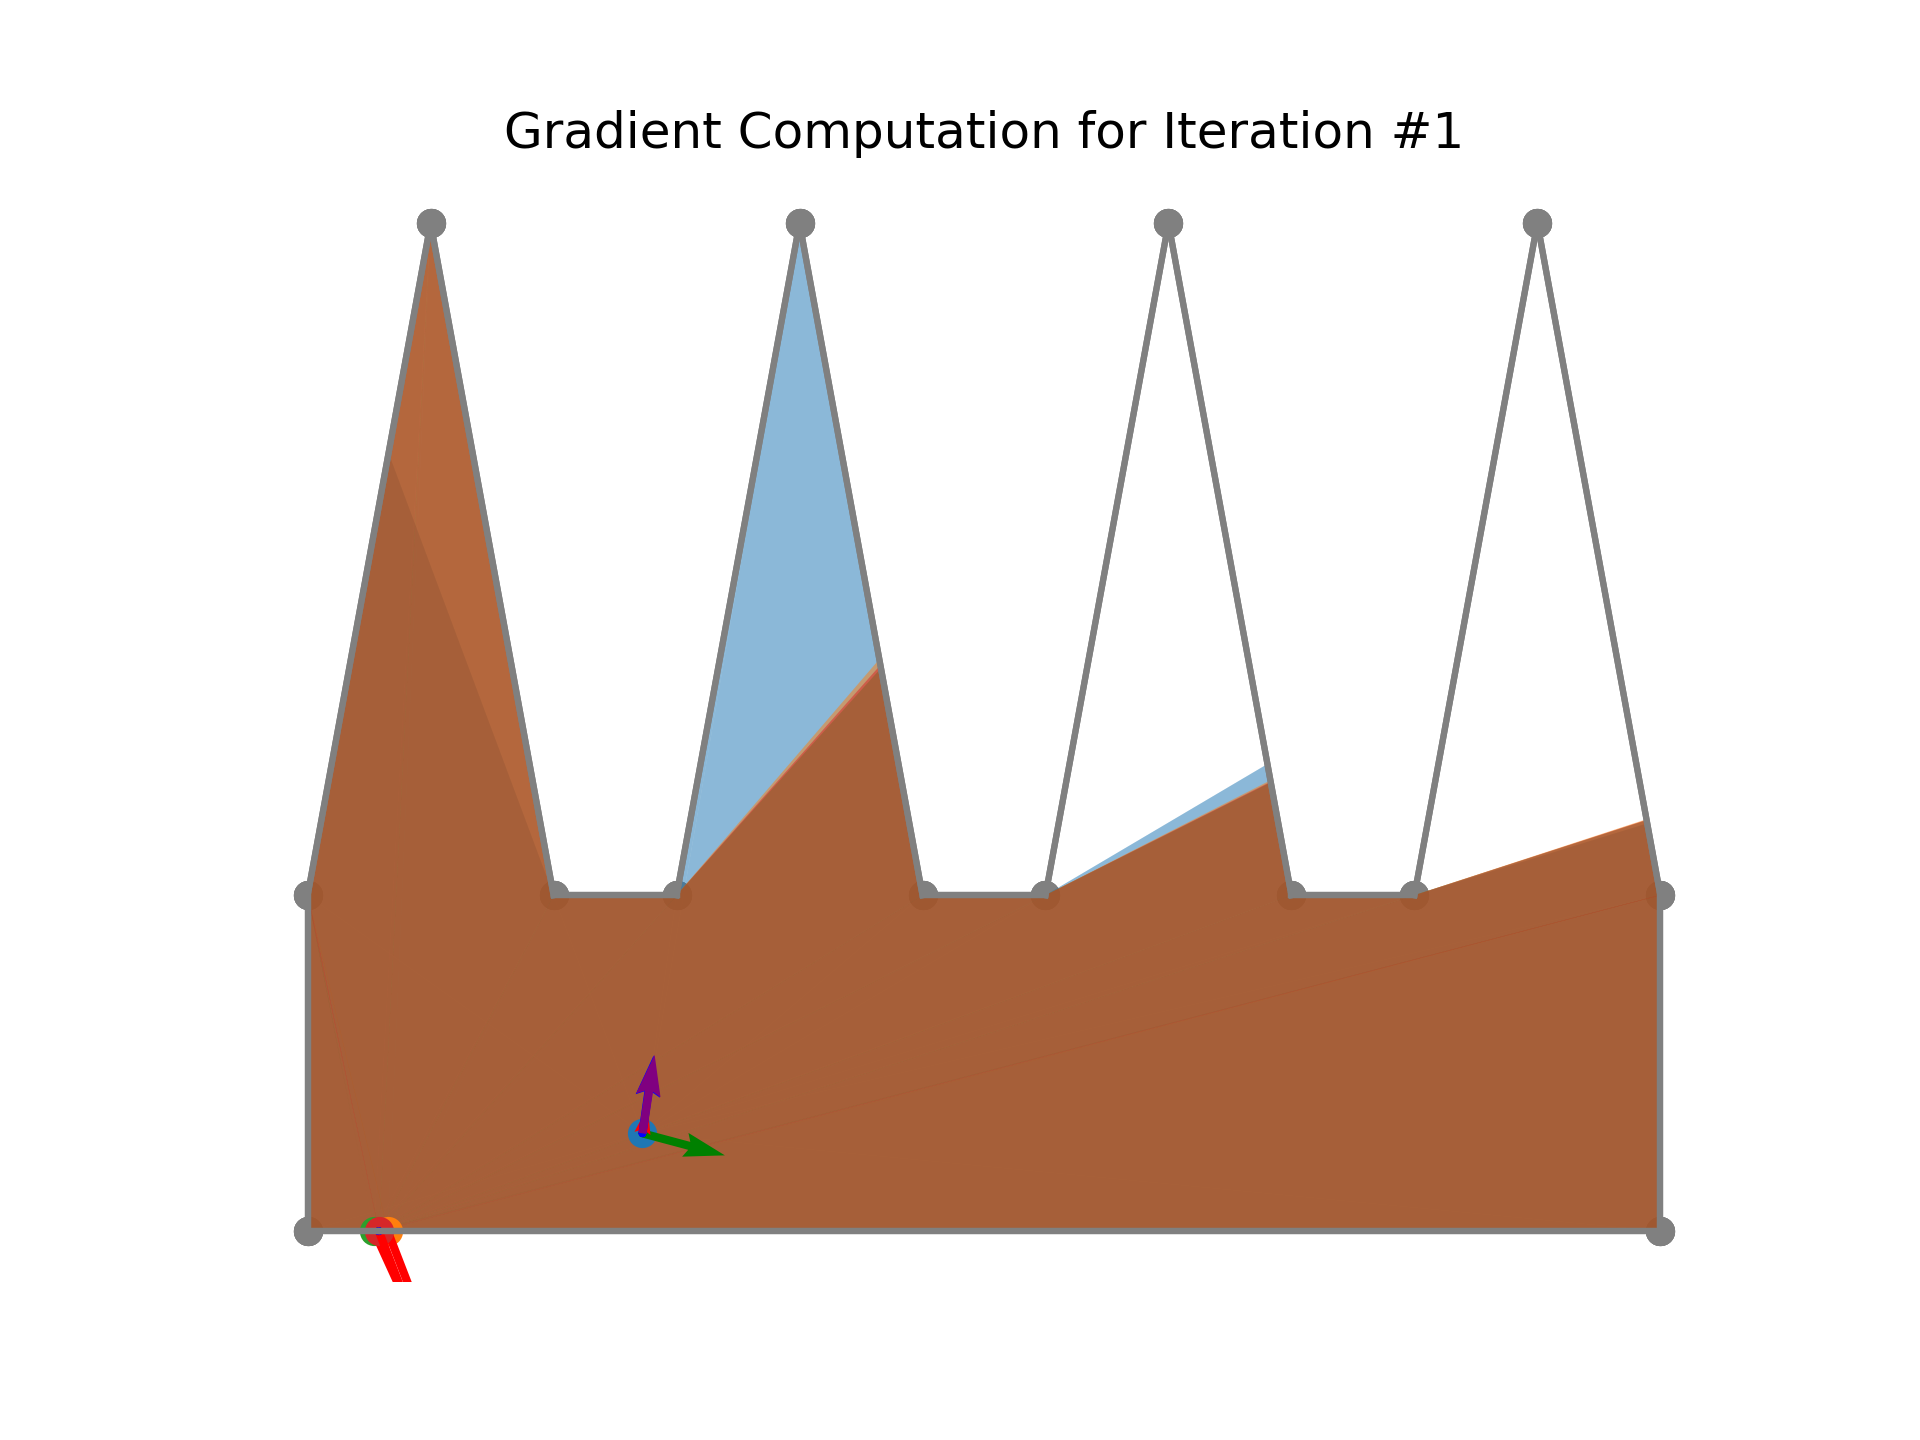
\includegraphics[width = \textwidth]{experiments/comb_no_capping_pos1.png}
        \caption{No pull onto the reflex vertex, iteration 1. The guard is drawn closer to the reflex vertex.}
        \label{fig:no_cap_pos1}
    \end{subfigure}
    \vfill
    \begin{subfigure}{0.45\textwidth}
        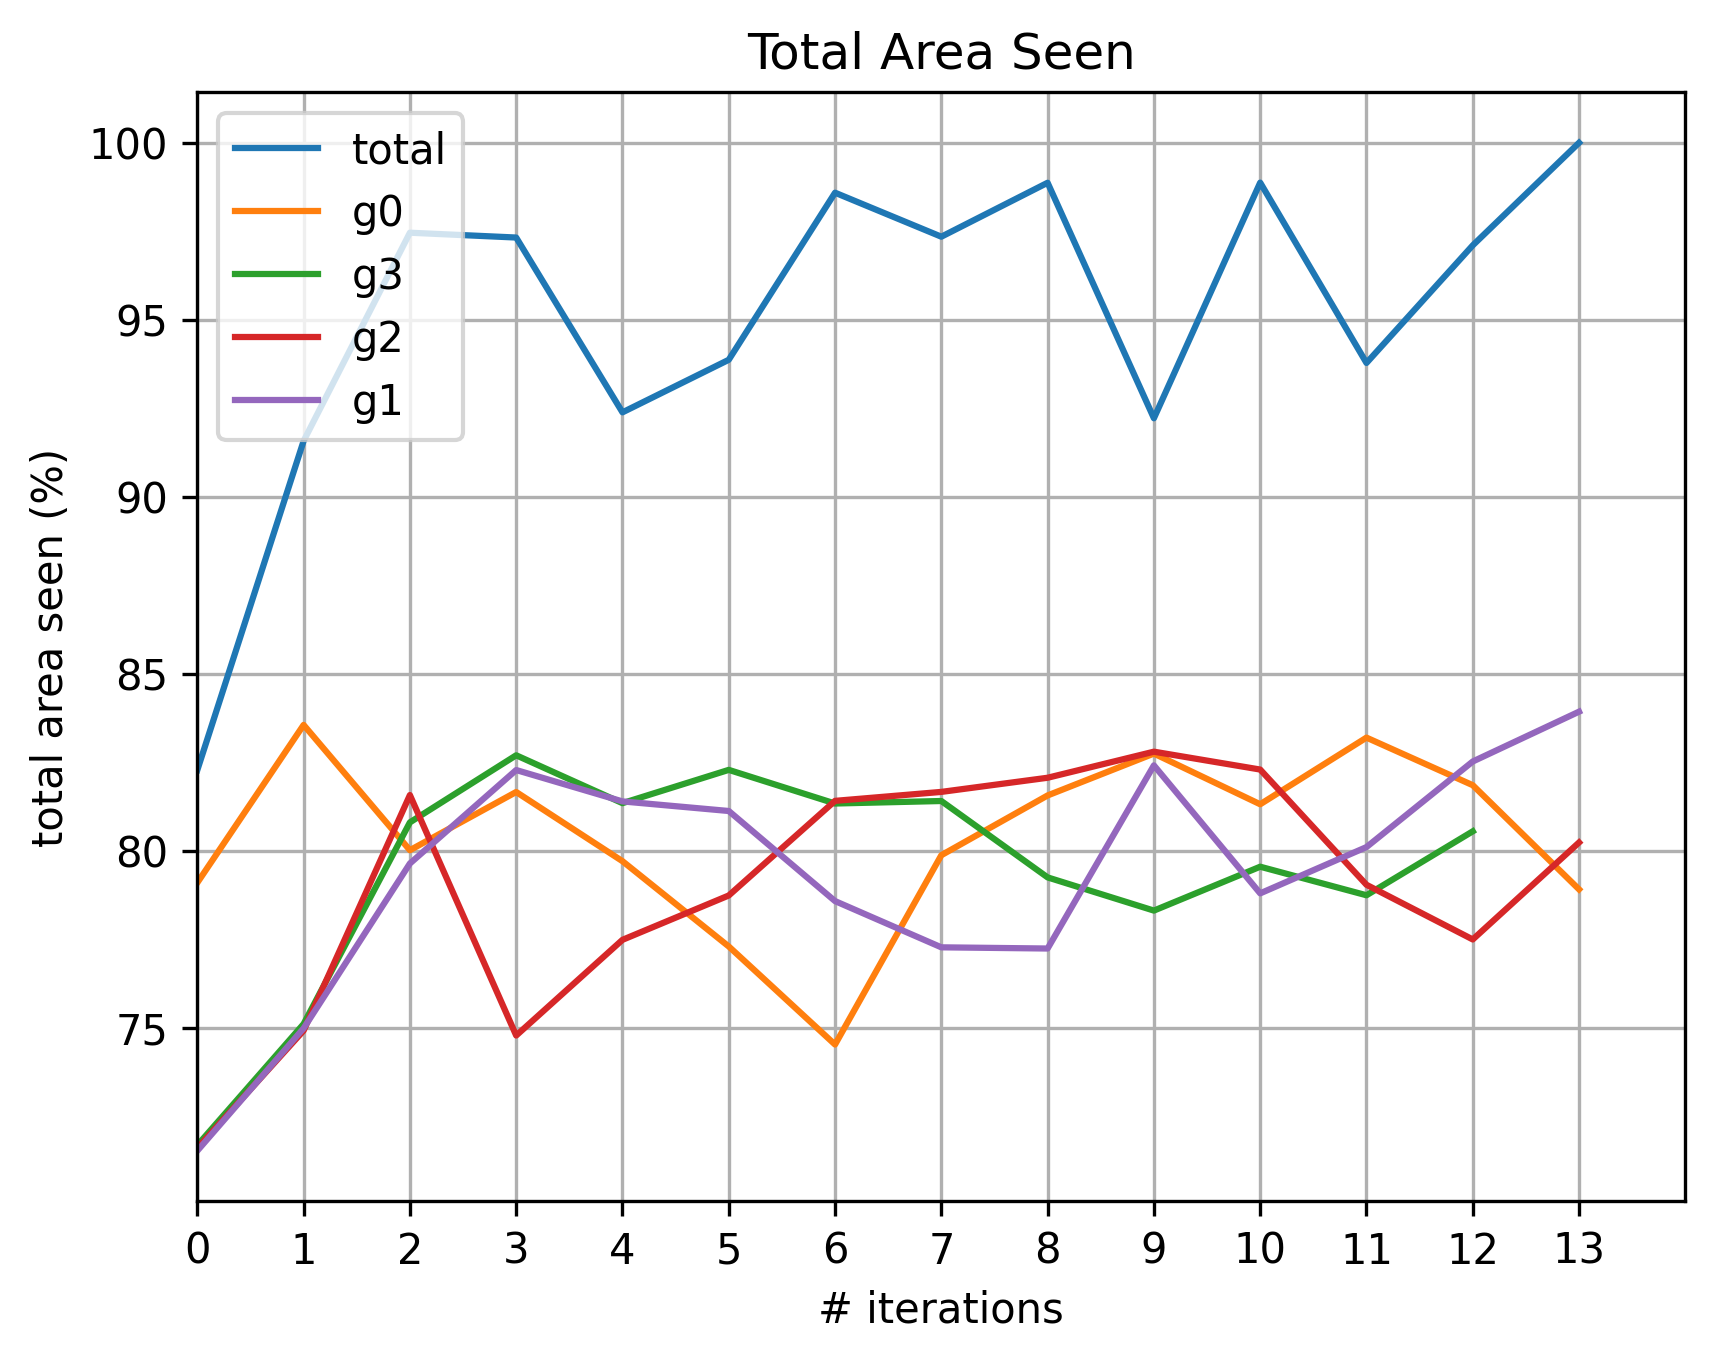
\includegraphics[width = \textwidth]{experiments/area_comb_capping.png}
        \caption{Seen area for all heuristics.}
        \label{fig:area_all_cap}
    \end{subfigure}
    \hfill
    \begin{subfigure}{0.45\textwidth}
        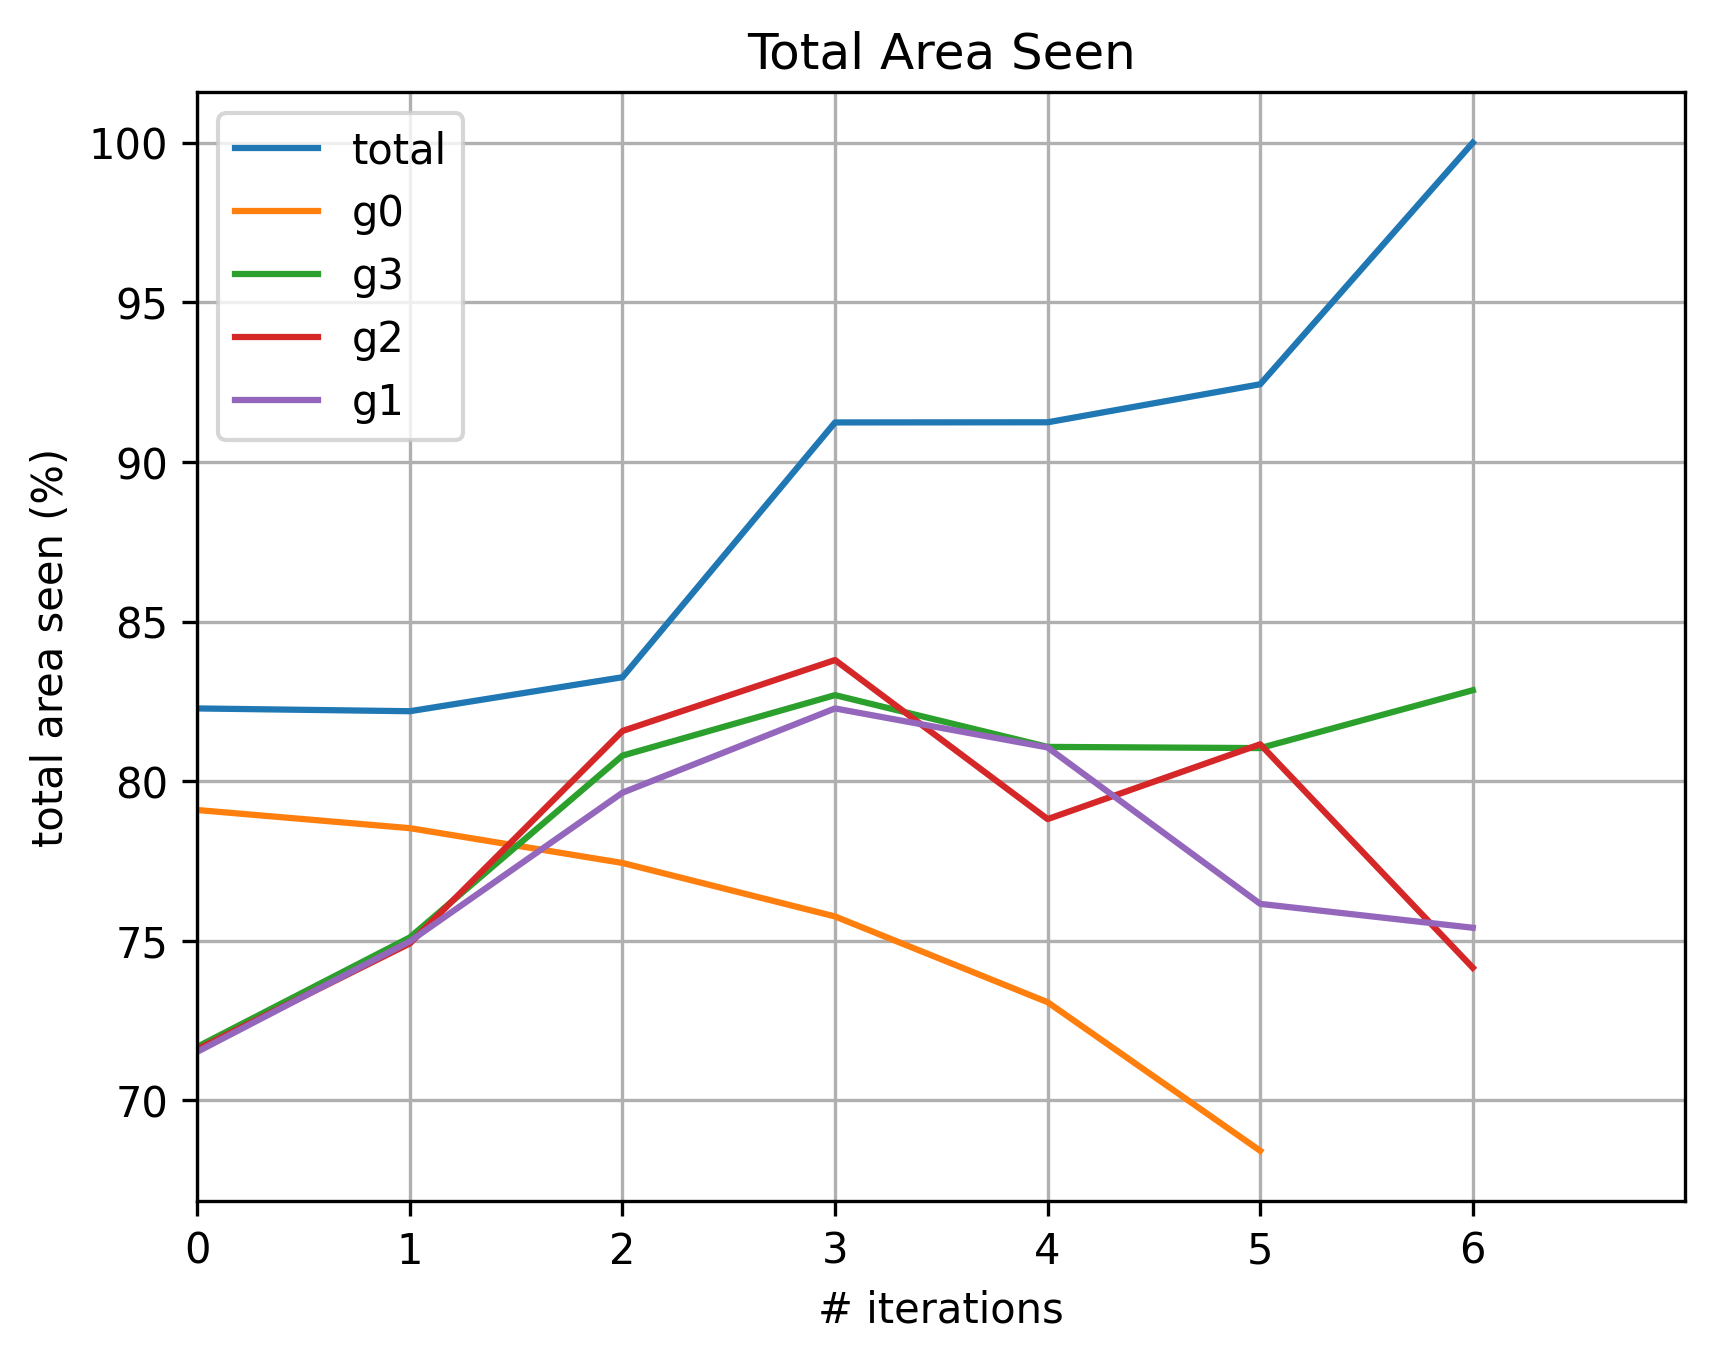
\includegraphics[width = \textwidth]{experiments/area_comb_no_capping.png}
        \caption{Seen area without pull capping.}
        \label{fig:area_no_cap}
    \end{subfigure}
    \caption{Example of different behaviours of a guard with and without its reflex vertex pull capped in a comb polygon with four teeth.}
    \label{fig:no_capping}
\end{figure}


% - momentum
- reflex vertex pull
    % - onto reflex vertex
    % - pull Capping
% - line search
- reflex area
- hidden gradient
- angle behind reflex vertex
- greedy initialisation